\documentclass[a4paper]{article}
\usepackage{graphicx}
\graphicspath{/home/angelo/Documents/Uni/Courses/Advanced Statistics and programming/Assignments/assignment2/} 
\usepackage{mathtools}
\usepackage[a4paper, total={5in, 6.5in}]{geometry}
\usepackage{color}
\usepackage{tikz}
\usepackage{lipsum}
\usepackage{geometry}
\geometry{a4paper, left=2.5cm, top=2.5cm, bottom=2.5cm, right=2.5cm}
\usepackage{changepage}
\usepackage{booktabs}
\usepackage[font=small]{caption}
\DeclareCaptionFormat{mycaptionfont}{\fontsize{12}{13}\selectfont#1#2#3}
\usepackage{threeparttable}
\usepackage{ntheorem}
\usepackage{caption}
\usepackage{wrapfig,lipsum,booktabs}
\usepackage{listings}
\usepackage{pdflscape}
\captionsetup{format=mycaptionfont}
\usepackage{subcaption}
\theoremseparator{:}
\usepackage{lscape}
\usepackage{rotating}
\usepackage[utf8]{inputenc}
\newtheorem{hyp}{Hypothesis}
\usetikzlibrary{shapes,decorations,arrows,calc,arrows.meta,fit,positioning}
\tikzset{
    -Latex,auto,node distance =1 cm and 1 cm,semithick,
    state/.style ={ellipse, draw, minimum width = 0.7 cm},
    point/.style = {circle, draw, inner sep=0.04cm,fill,node contents={}},
    bidirected/.style={Latex-Latex,dashed},
    el/.style = {inner sep=2pt, align=left, sloped}
}





\begin{document}

\title{ASAP Assignment 2}
\author{Angelo Barisano; 508903 }
\date{September 28th, 2022}
\maketitle

\newpage
\section{Difference in Difference}






\subsection{Task 1: Derive Diff-In-Diff Coefficients}
The canonical difference-in-difference equation is expressed in regression form (1-1): 

\

$(1-1) \ {y_{it}} = \beta_{0} + \beta_{1} D_i + \beta_{2} T_t+ \beta_{3} D_i T_t + \epsilon_{it}$

\

%, the individaul outcome of ${y_{it}}$ is defined by five terms:
%
%\begin{enumerate}
%	\item $\beta_{0}$; constant - will be cancelled out in later part
%    \item $\beta_{1} D_i$; treatment indicator - whether the subject is treated or not represented by either (D= 1$ | $D = 0)
%	\item $\beta_{2} T_t$; independent of the subject, the "event study" contains pre- and post-test measurements indicator for each subject
%	\item $\beta_{3} D_i T_t$; the interaction effect of the treatment indicator and the time indicator displays the assumed effect of the change from pre to post test in $T_t$ for an individual in the treatment or control - in case of treatment, this term falls out as the general assumtion of diff-in-diff pertains to the control being the same as the treatment. 
%	\item $\epsilon_{it}$; contains the disturbances
%\end{enumerate}


The terms in 2, 3, \& 4 are relevant in describing the potential outcome assumption in difference in difference analysis. Difference in difference suggests that we compare the difference between treatment and control before and after the treatment introduction (t = 0), shown as:

\

$
(1-2) \ [E(y_{T=1} | D=1) - E(y_{T=0} | D=1)] - [E(y_{T=1} | D=0) - E(y_{T=0} | D=0)]
$

\

Subsequetnly, the four outcomes described in (1-2) yield the following outcomes:

\begin{itemize}
\item $E = (y_{T=1} | D=1)$; Becasue we are observing the outcome for the post-(treatment) test for treatment group, this yields $\beta_{0}$, $\beta_{1}$, $\beta_{2}$, $\beta_{3}$
\item $E = (y_{T=0} | D=1)$; Because we are observing the outcome of the pre-(intervention) test for the treatment, this will yield $\beta_{0}$, $\beta_{1}$
\item $E = (y_{T=1} | D=0)$; Becasue we are observing the outcome for the post-(treatment) test for the control group, this yields $\beta_{0}$, $\beta_{2}$ 
\item $E = (y_{T=0} | D=0)$; Because we are observing the outcome of the pre-(intervention) test for the control, this will yield $\beta_{0}$
\end{itemize}

Note that the disturbance term ($\beta_{0}$)is left out as it is assumed to be independent of the treatment allocation; as such we will ignore it here. 
Additionally, the constant is present in all four outcomes; thus, it also technically cancels out in the following equation. This originates from the assumption that the covariates measurements in pre- and post test yield the same results for both treatment and control subjects. Equivalently, by substitution the aforementioned outcomes into (1-2), the following results can be deduced (excluding the constant):

\

$
(1-3) \ E(y_{it}) =  [E(y_{T=1} | D=1) - E(y_{T=0} | D=1)] - [E(y_{T=1} | D=0) - E(y_{T=0} | D=0)]
$

\

$
 (=) \ E(y_{it}) = [(\beta_{1} + \beta_{2} + \beta_{3}) - (\beta_{1})] - [(\beta_{2})]
$

\

$
(=) \ E(y_{it}) = (\beta_{2} + \beta_{3}) - \beta_{2} = \beta_{3}
$




% Table created by stargazer v.5.2.3 by Marek Hlavac, Social Policy Institute. E-mail: marek.hlavac at gmail.com
% Date and time: Fri, Sep 23, 2022 - 20:25:57
\begin{table}[!htbp] 
\begin{adjustwidth}{-0cm}{-0cm}
\begin{threeparttable}
\small
\captionsetup{font=small, justification=raggedright,singlelinecheck=false}
  \caption{Descriptive Statistics of Numeric Indepdenent and Dependent Varaible} 
  \label{} 
\begin{tabular}{@{\extracolsep{5pt}}lccccccc} 
\\[-5.8ex]\hline 
\hline \\[-1.8ex] 
Statistic & \multicolumn{1}{c}{Mean} & \multicolumn{1}{c}{St. Dev.} & \multicolumn{1}{c}{Min} & \multicolumn{1}{c}{Pctl(25)} & \multicolumn{1}{c}{Median} & \multicolumn{1}{c}{Pctl(75)} & \multicolumn{1}{c}{Max} \\ 
\hline \\[-1.8ex] 
Unemp. Rate & 6.762 & 1.462 & 2.600 & 5.700 & 6.800 & 7.700 & 11.400 \\ 
Number Children & 1.193 & 1.382 & 0 & 0 & 1 & 2 & 9 \\ 
Family Income & 15,255.320 & 19,444.250 & 0.000 & 5,123.418 & 9,636.664 & 18,659.180 & 575,616.800 \\ 
Earnings & 10,432.480 & 18,200.760 & 0.000 & 0.000 & 3,332.180 & 14,321.220 & 537,880.600 \\ 
Age & 35.210 & 10.157 & 20 & 26 & 34 & 44 & 54 \\ 
Education (y) & 8.806 & 2.636 & 0 & 7 & 10 & 11 & 11 \\ 
Unearned Income & 4.823 & 7.123 & 0.000 & 0.000 & 2.973 & 6.864 & 134.058 \\ 
\hline \\[-3.6ex] 
\end{tabular} 
\begin{tablenotes}[para,flushleft]
      \small
      \item\textit{Notes:} N = 13746
    \end{tablenotes}
\end{threeparttable}
\end{adjustwidth}
\end{table}

% Table created by stargazer v.5.2.3 by Marek Hlavac, Social Policy Institute. E-mail: marek.hlavac at gmail.com
% Date and time: Fri, Sep 23, 2022 - 21:38:43
% Requires LaTeX packages: dcolumn 
\begin{table}[!htbp] 
\begin{adjustwidth}{-0cm}{-0cm}
\begin{threeparttable}
\small
\captionsetup{font=small, justification=raggedright,singlelinecheck=false}
  \caption{Diff-in-Diff Matrix} 
  \label{} 
\begin{tabular}{@{\extracolsep{8pt}}lccccccc} 
\\[-5.8ex]\hline 
\hline \\[-1.8ex]
\multicolumn{2}{c}{}  & \multicolumn{2}{c}{Earning}  & \multicolumn{2}{c}{Family Income} & \multicolumn{2}{c}{Work Participation} \\ 
\multicolumn{1}{c}{} & \multicolumn{1}{c}{dperiod} & \multicolumn{1}{c}{Childless} & \multicolumn{1}{c}{Children} & \multicolumn{1}{c}{Childless} & \multicolumn{1}{c}{Children} & \multicolumn{1}{c}{Childless} & \multicolumn{1}{c}{Children} \\ 
\hline \\[-1.8ex] 
\multicolumn{1}{c}{Before} & 1 & 14,203.900 & 7,290.380 & 19,159.190 & 12,140.900 & 0.580 & 0.450 \\ 
\multicolumn{1}{c}{After} & 2 & 13,507.900 & 8,277.200 & 18,218.950 & 13,111.690 & 0.570 & 0.480 \\ 
\multicolumn{1}{c}{Difference} &  & -696.000 & 986.810 & -940.240 & 970.800 & -0.010 & 0.030 \\ 
\hline \\[-3.6ex] 
\end{tabular} 
\begin{tablenotes}[para,flushleft]
      \small
      \item\textit{Notes:} N = 5927 Childless; N = 7819 Has one or more Children.
    \end{tablenotes}
\end{threeparttable}
\end{adjustwidth}
\end{table}

\subsection{Task 2: Provice Graphical "evidence" for the presence of the DiD effect}

\begin{wrapfigure}{L}{9cm}
\centering
\begin{subfigure}[b]{0.48\textwidth}
    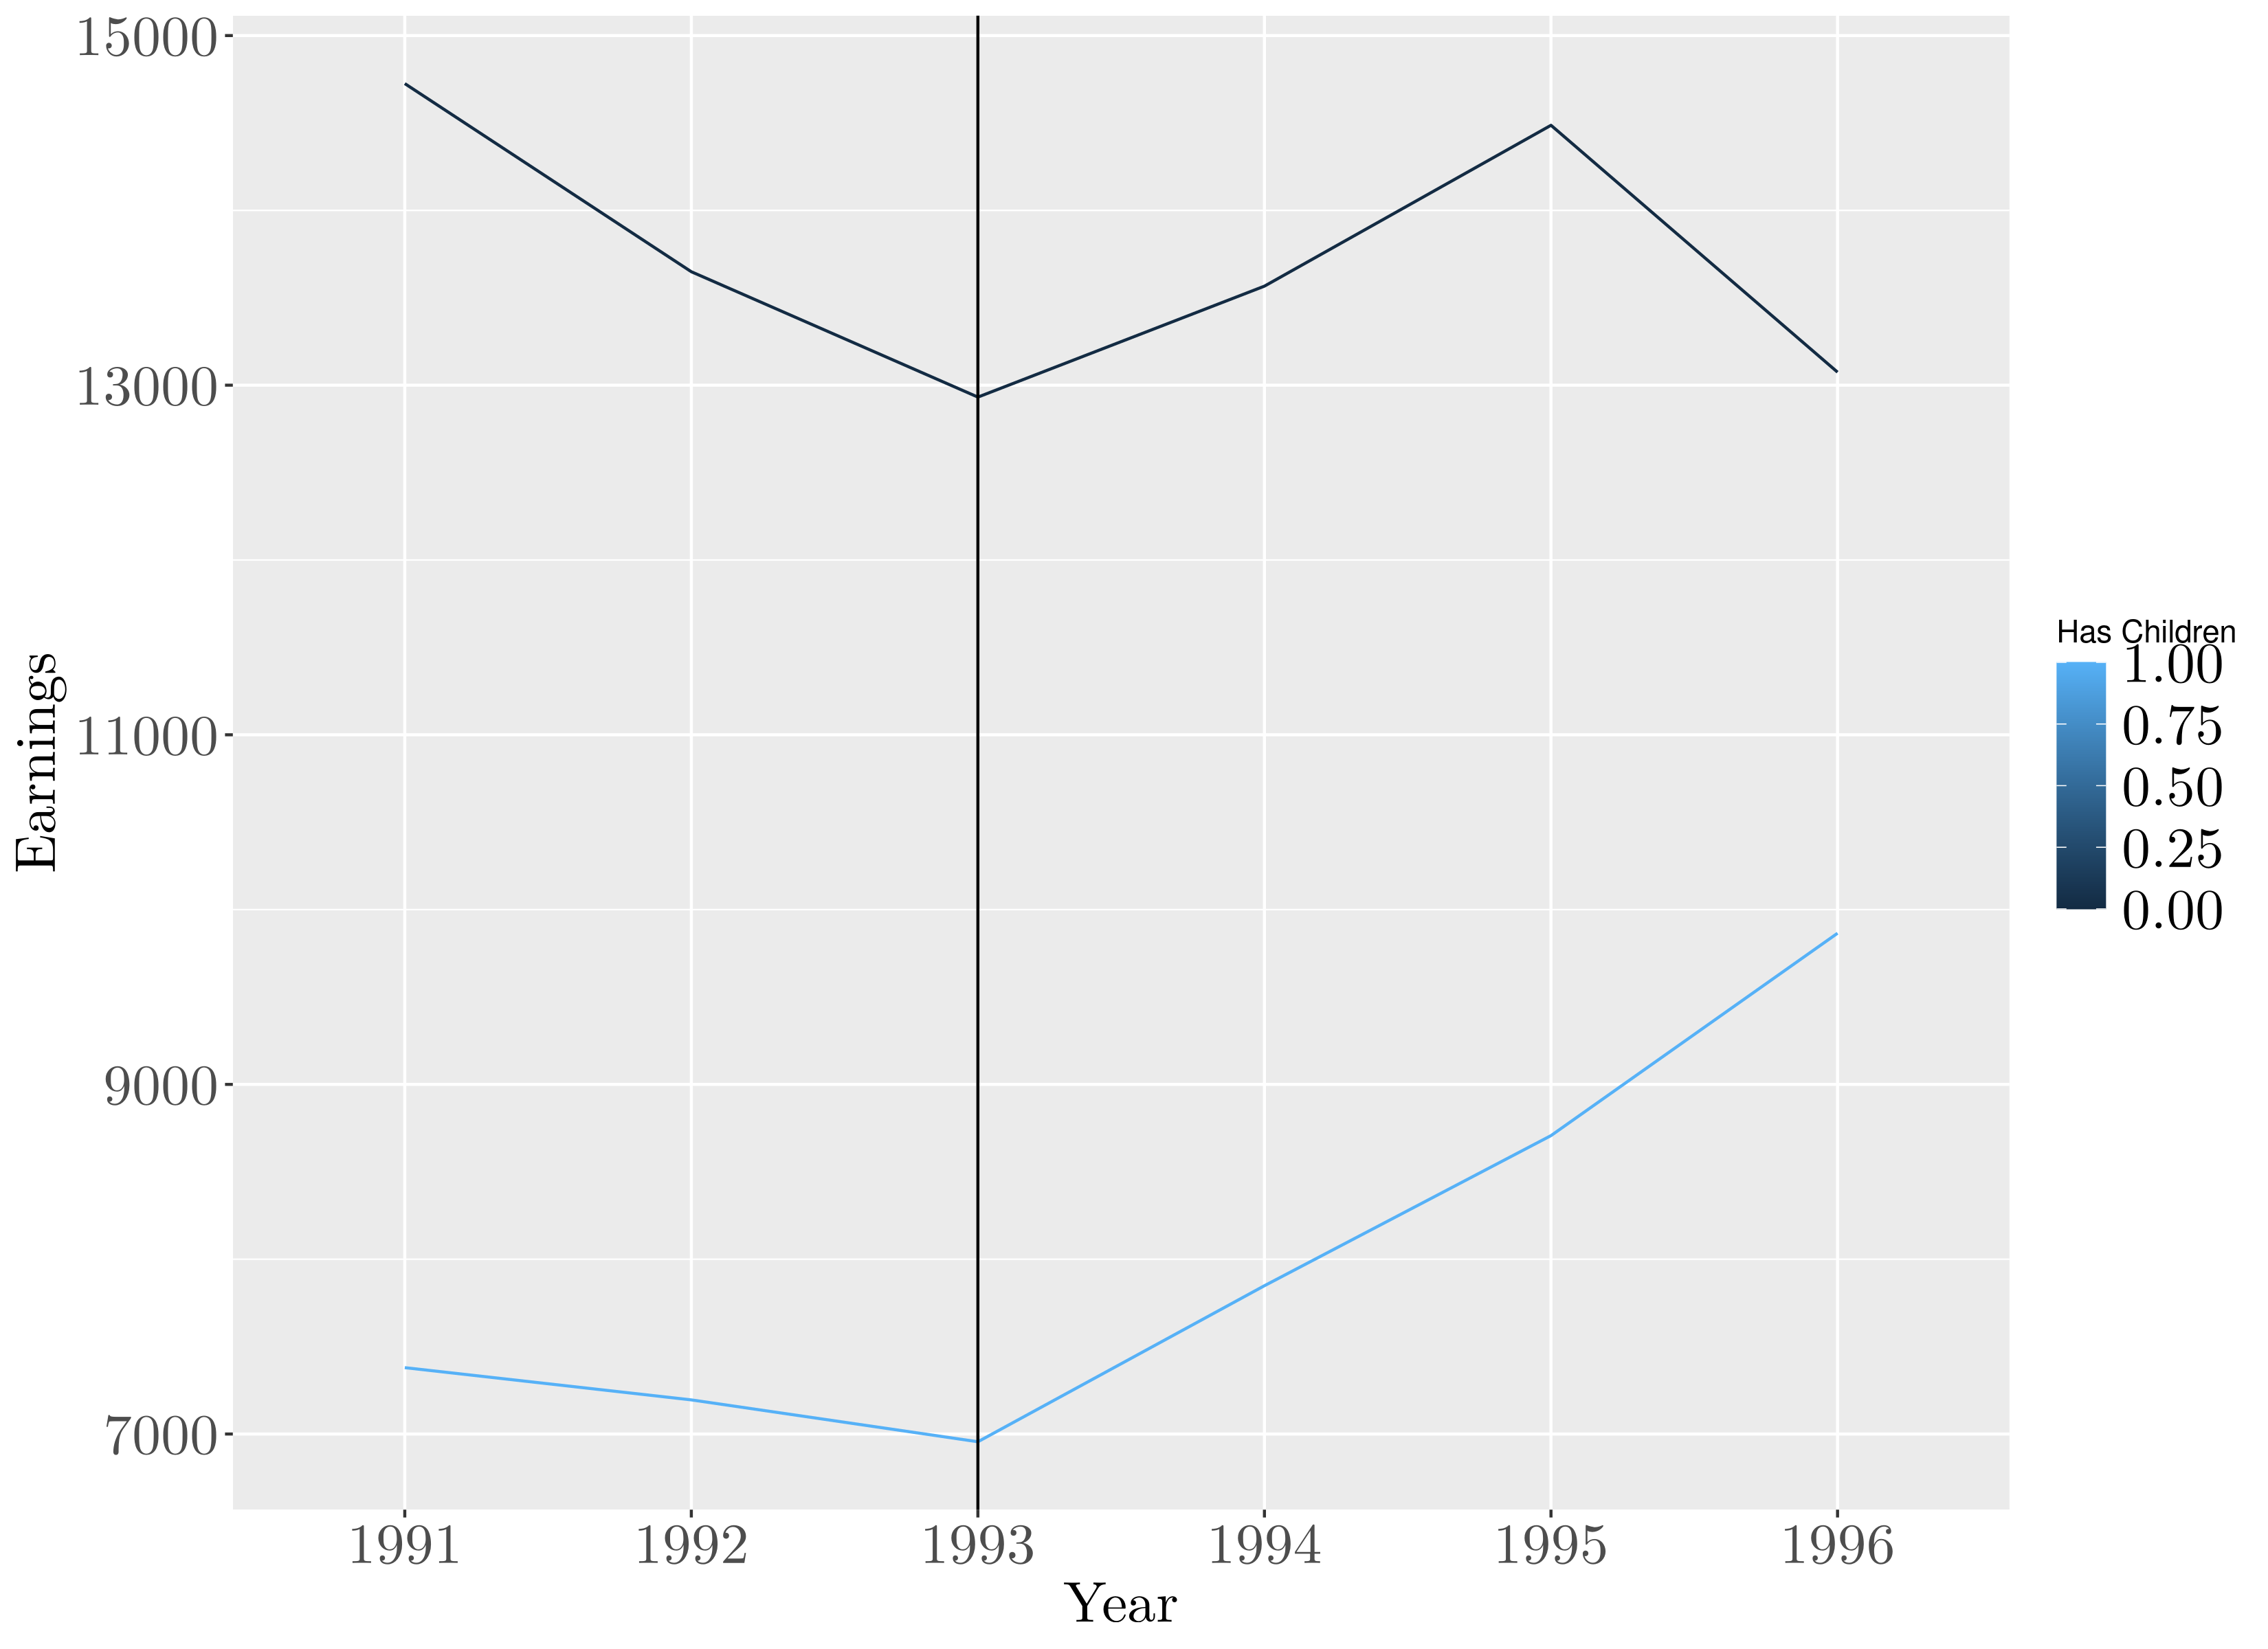
\includegraphics[width=.95\linewidth]{"/home/angelo/Documents/Uni/Courses/Advanced Statistics and programming/Assignments/assignment2/Graphics/task2_earn_did.png"} 
   \caption{Annual Earnings by Females with(out) Children}
   \label{fig:Ng2}
\end{subfigure}

\begin{subfigure}[b]{0.48\textwidth}
    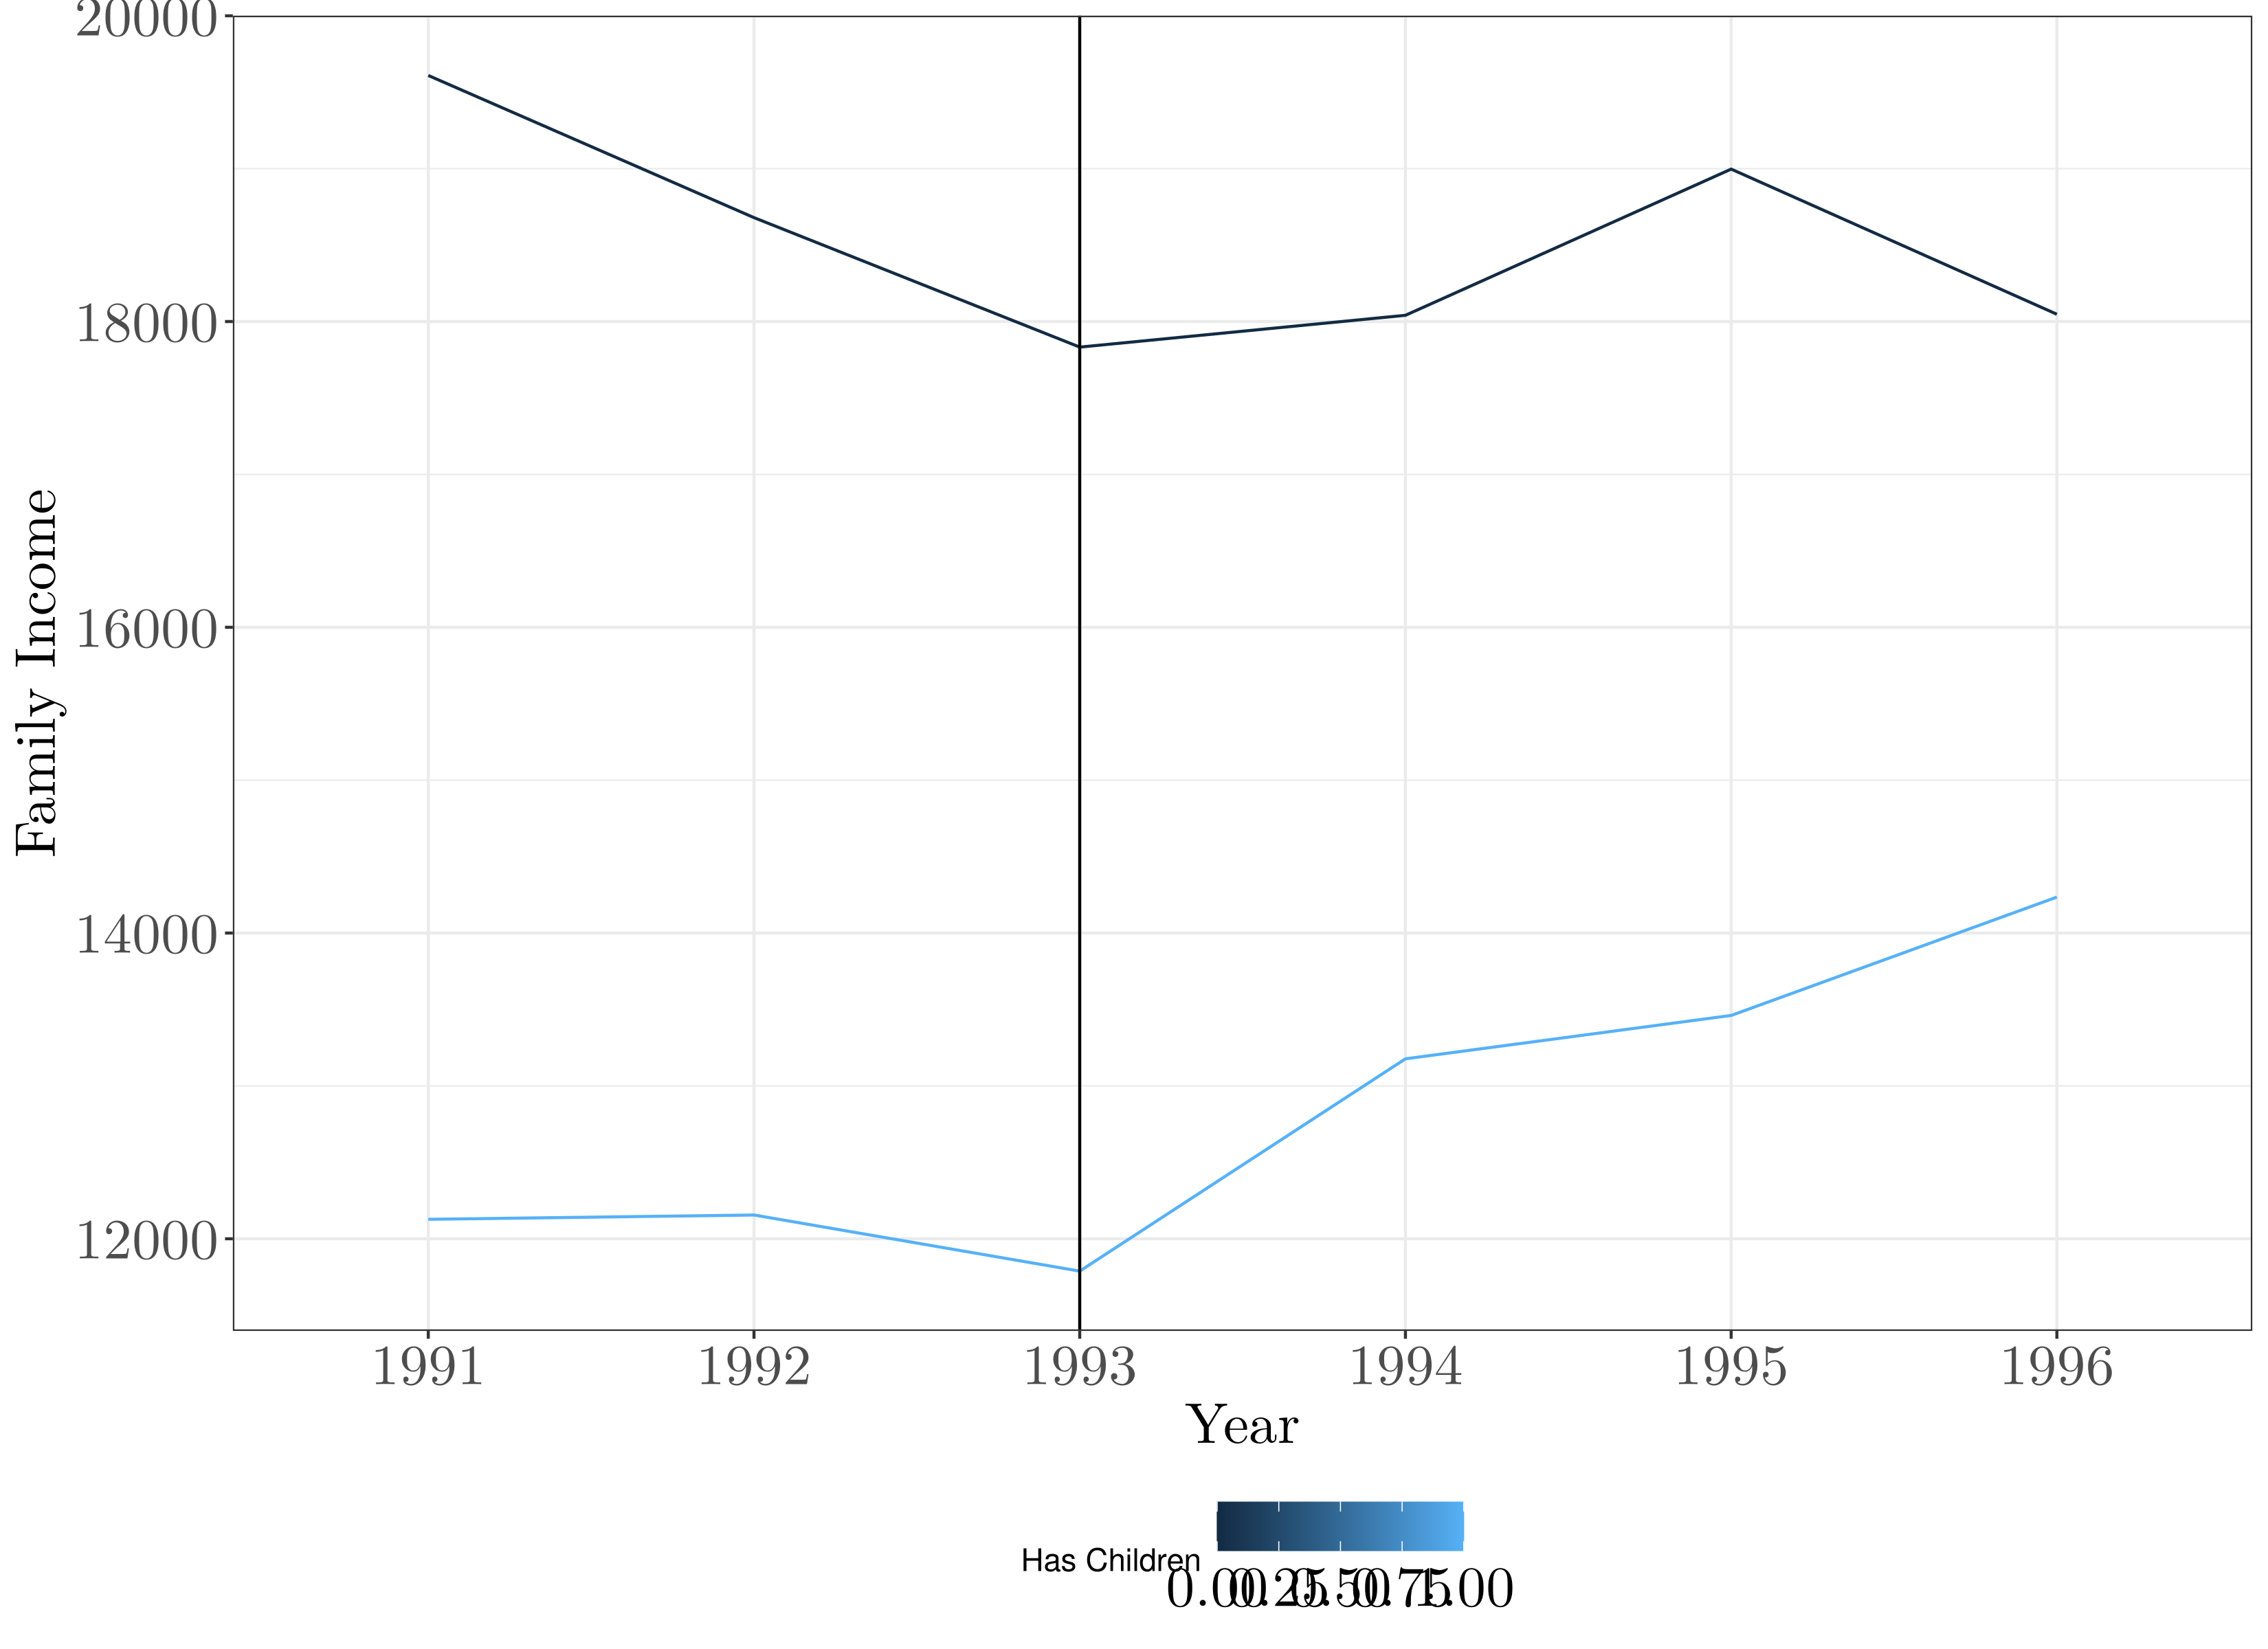
\includegraphics[width=.95\linewidth]{"/home/angelo/Documents/Uni/Courses/Advanced Statistics and programming/Assignments/assignment2/Graphics/task2_finc_did.png"} 
   \caption{Family Earnings Earnings by Females with(out) Children}
   \label{fig:Ng2}
\end{subfigure}

\begin{subfigure}[b]{0.48\textwidth}
    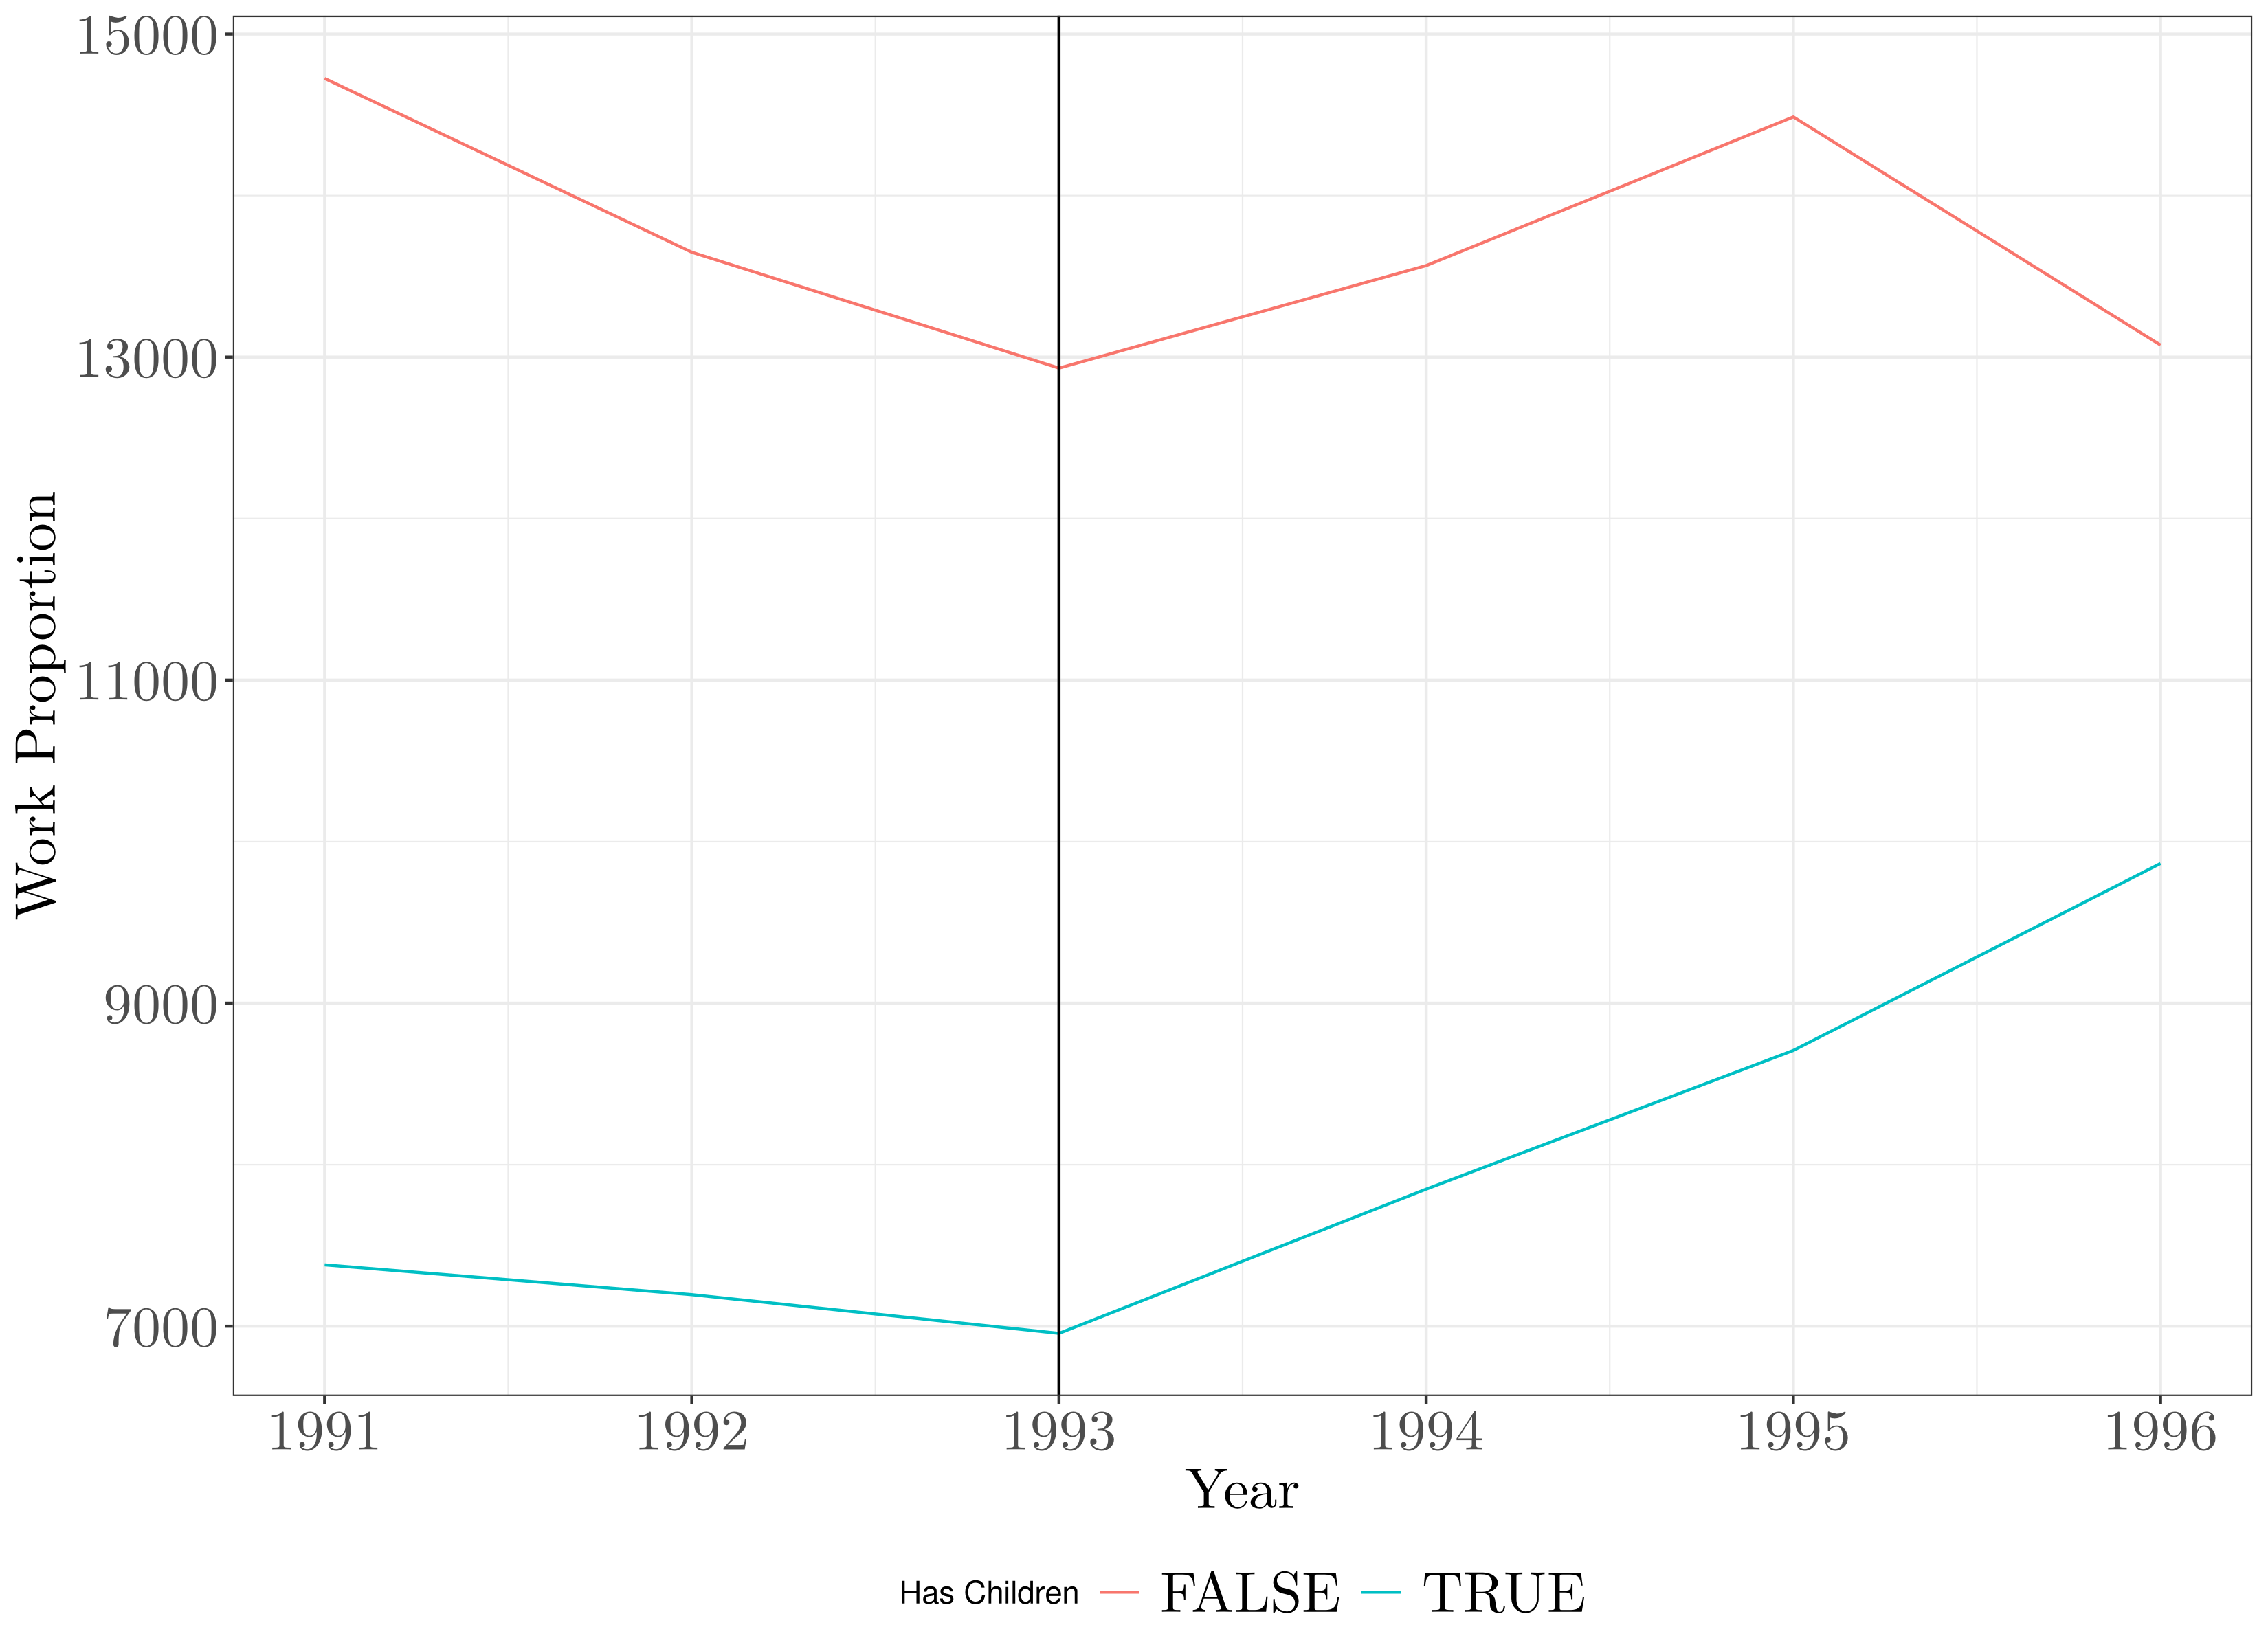
\includegraphics[width=.95\linewidth]{"/home/angelo/Documents/Uni/Courses/Advanced Statistics and programming/Assignments/assignment2/Graphics/task2_work_did.png"}  
   \caption{Work Participation by Females with(out) Children}
   \label{fig:Ng2}
\end{subfigure}
\captionsetup{justification=centering}
\caption{Pre-Post Intervention of EICT Credit for Women with(out) Children}
\end{wrapfigure}

Figure 1 displays the outcomes for both treatment and control group for earnings (earn), family income (finc), and work-participation indicator (work) over the period form 1991 to 1996. THe treatment in this case is defined as a binary state of females with children (one or many) (D = 1) and females without children (D = 0). The tax credit (EITC) is assumed to be introduced on the 1st of January 1993.
\indent Figure 1 a) displays the development of earnings and the introduction of the EITC is marked by the vertical line (as in the other graphics). Females without children earned considerably more on average than females with children (pre-period $mean$ = 7290.38) during the pre-period, starting out at slightly less than \$14800 and dropping to \$13000 at its lowest, with and average pre-intervention earnings of \$14203.90. Overall, both groups displayed a downward trend before 1993. After 1993, the supposed introduction of the EITC, both groups experienced an increase in earnings; However, the childless group did not display a continous increase in earnings (post-period $mean$  = 13507.90) when compared to females with children (post-period $mean$  = 8277.20). This might suggest that the introduction of the  EITC is associated to the average earnings of women with children but not for women without children.
\indent Figure 1 b) shows the same features as the plot before but the outcome is now Family Income (numbers discussed in exercise 3 and 4). Overall, the general trend is similar for both groups as in Figure 1 a); it may be noted that the trend for females with child is less pronounced than in a). Nonetheless, the conclusion is the same as in a): During the pre-period, childless women earned more, but drecreased stronger than women with children, while the post treatment movement is not continous (dropping to pre treatment levels) for childless women when compared to women with children, which experience continous growth on average.
\indent Figure 1 c) displays workparticipation of females with and without children.Again, childless women start out higher at around 54\% workparticipation vs 46\% workparticipation for women with children. Moreover, the trends are somewhat comparable to the two preceeding graphics, as females with children display an increase to 50.3\% (and then a slight drop in the following year), while childless women tend to decrease: As such, women with children again experience an average net gain in work participation during the post period, while childless women drop below pre-treatment levels. 









\subsection{Task 3: Summary Statistics for data}
The dataset is not balanced and we cannot assure that it is fixed. Nonetheless, for the purpose of this exercise, it is assumed that it is balanced and fixed. The data contains yearly records from 1991 to 1996; the reported values per variable are thus averages over all six years. A total of 13746 records were made, split by year into 2610, 2449, 2342, 2255, and 2085 observations respectively. Of the total 13746 observations, 7819 have one or more children, and 5927 have no children.\footnote{additional summary statistics can be found for women with and without children in Appendix 4.1}. Of the relevant outcome variables (earnings, family income, work participation), the average family income was \$15255.32 ($std$ = 19444.24, $median$ = 9636.66). This large spread around the mean was partially addressed by Figure 1 a) displaying a large difference between women with and without children; this suggests a strong heterogenity in the data wrt. to the outcomes. Additionally, as was to be expected by the financial nature of family income, there is a severe positive skewness of 7.06. Earnings displays a similar pattern as family income ($mean$ = 10432.48, $std$ = 18200.76, $median$ = 3332.18 $skew$ = 6.766), which is supported by Figure 1 b). As expected, earnings and family income correlate strongly with a Pearson correlation coefficient of .93 ($p$ $<$ 0.001); thus, earnings and family income are assumed to behave similarly as outcome variables. Finally, work participation shows that 51.3\% of records over all six years are in employment (std. and median have no meaning here as it is a binary variable). Considering possible covariates, the average years in education is 8.8 ($std$ = 2.636), with 11 years in the median. On average, per year, one women had 1.19 children ($std$ = 1.382, $median$ = 1), with 56.9\% of respondents having one child or more (N = 7819). Of the respondents 60\% were people of colour. Unemployment rate by state was on average 6.76\% ($std$ = 1.462, $median$ = 7.7) and unearned income at \$4823 ($std$ = 7123, $median$ = 6864)

\subsection{Task 4: Diff in Diff Matrix}


Table 2 reports the pre-post intervention averages for the two groups - Women with children and women without children - for earnings, family income, and work participation proportion. As shown in Figure 1 a) childless women have on average higher earnings in both pre- and post period than women with children. However, only women with children show a positive average gain over the post intervention period of \$986.82, when compared to the average over the pre treatment period, while childless women even drop in earnings in the post period. Using formula (1-2) this results in a $naive$ DiD effect of \$1682.81 for women with children. Again, a similar observation can be made for family income which displays a DiD of \$1911.04. Finally, work participation also followed the trend observed in Figure 1 c), suggesting a DiD effect of 0.04 (or 4\% point gain ov women with children over childless women). Please note that these are just pre-post averages of the groups, complementing the descriptive statistics from part 2-3
\textbf{maybe describe a bit more}

\subsection{Task 5: Analyze the DiD regression}
\textbf{ADD POPULATION REGRESSION}

\textbf{Tutoial 1 plot for heteroscedasiticty fitted vs standardized residuals}

\paragraph{No model without theory} Considering possible covariates, earnings, workparticipation, and family income all tend to vary with age (inverted u). Moreover, higher unemployment implies more labour supply and suppression of wages, family income and (obviously) work participation. Furthermore, higher education positively correlates with earnings, family income, and workparticipation. Finally, the US is known for racial tensions; people of colour tend to show lower incomes and lower work pariticpation in general. 

\textbf{CITE A COUPLE OF THINGS FOR THIS!!}

\paragraph{Results} For brevity reasons, Table 3 contains models for all three outcome variables, with the first model per outcome (1, 4, 7) containing a baseline model with only covariates. Models 2, 5, 8 contain only the DiD effects, and Models 3, 6, 9 contain the full model respectively. 

\indent Considerig earnings, the covariate model (1) shows only that nonwhite (indicator variable) ($\hat{\beta}$ = -2037.990, $p$ $<$ 0.001) and age ($\hat{\beta}$ = 96.038, $p$ $<$ 0.01) are significant. Overall, this model explains 0.6\% of the variation in earnings. Proceeding to only the DiD effect (model 2), as expected, women with children earn on average \$8596.33 ($p$ $<$ 0.01) less than childess women.\footnote{Note: the period indicator is not really relevant in such an exercise as compares the total trend change for two converging groups $y$} Subsequently, the value from Table 2 for the DiD effect is statistically significant at conventional levels, suggesting that women with children gain a \$1682.81 ($p$ $<$ 0.01) in the post treatment/intervention period (compared to pre period) (1993 $<$) when compared to childless women; overall explaining 2.6\% of the total variation in earnings. This effect is important to be examined more closely: As implied in task 4, while childless women on average earn \$ 8596.33 more than women with children, childless women (see Table 2) drop by \$696 when comparing the before and after period, while women with children increased. These two effects cancel each other out out, most likely leading to the insignificant period coefficient. Moreover, this suggests that the comparison groups (women with vs women without children) are not comparable; as such we will not be able to discern causality from this exercise. Finally, model (3) considers the full model. Focusing on the DiD effect after including covariates, we see a slight increase in the coefficient ($\hat{\beta}$ = 1722.360, $p$ $<$ 0.01) with stable standard errors; suggesting that women with children in the post period earn \$1722.36 more than childless women. However, the inclusion of the covariates does not suggest a considarable change in the direction of the outcome. 
\indent Moving to family income as an outcome, a similar insights can be drawn. However, now all covariates are significant - model explaining 1.2\% of the variation in family income. Again, the DiD effect alone in model (5) is significant ($\hat{\beta}$ = 1911.04, $p$ $<$ 0.01); suggesting again that women with childrens' familiy income increases by \$1911.04 after the intervention (when compared to the pre-period) when compared to childess women. Additionally, women with children, again, have a lower family income of \$-8929.33 ($p$ $<$ 0.01). This model explains 2.2\% of the total variation in family income. The inclusion of covariates does not change this insight dramitically; womens' with children family income still improve significantly by \$2006.06 during the post period when compared to childess women and its coefficeint also increases, but the insight is the same as before ($p$ $<$ 0.01). 
\indent Finally, considering work participation; the covariates in model (7) are all significant at the conventional level in predicting work participation, explaining 1.9\% of total variation in this outcome. As observed during task 1 through 4, work participation rises for women with children during the post intervention period (model 8) ($\hat{\beta}$ = 0.031, $p$ $<$ 0.1); however, the effect is only marinally significant. As was to be expected, women with children show a significantly lower work participation ($\hat{\beta}$ = -0.159, $p$ $<$ 0.01) when compared to childless women (15.9\$ less). When combining covariates and the base model in model (9), the overall trend is the same as in the aforementioned models. The coefficient for the DiD effect rises to 0.033 ($p$ $<$ 0.1), but is still only marginally significant.
Thus, overall, the inclusion of the covaraites does increase the coefficints of all three DiD effects, but only marginally. This means that the overall effect, or direction of the coefficicients was not changed drastically. Moreover, the inclusion of the covariates shows that the standard errors are stable across all models, suggesting no probelm with multicollinearity. 
\paragraph{Robustness Tests} Overall, due to the standard errrors between the models for each outcome variable respectively staying stable, this suggests that there is generally less necessity to include robust standard errors. Running the Breusch-Pagan test on all models in Table 3 - only model (1) and model (4) (both covariate-only models) fail to reject the null hypothesis of heteroscedasitc residuals. Finally, Table 11 in the appendix reports robust standard errors (white) and clustered by state. Overall, the standard errors are stable across models, which suggests, that there is little need to use robust standard errors.\footnote{Stability in coefficients also implies no multicollinearity; additionally, standardized coefficeints are not of use here becasue we are interested in the DiD effect.} 


\begin{landscape}
% Table created by stargazer v.5.2.3 by Marek Hlavac, Social Policy Institute. E-mail: marek.hlavac at gmail.com
% Date and time: Wed, Sep 28, 2022 - 18:35:54
\begin{table}[!htbp] \centering 
\begin{adjustwidth}{1.25cm}{-0cm}
\begin{threeparttable}
\small
\captionsetup{font=small, justification=raggedright,singlelinecheck=false}
\caption{\textsc{Non-Robust Regression Results Part 3}}
\centering 
  \label{}
\small 
\begin{tabular}{@{\extracolsep{-2pt}}lccccccccc} 
\\[-5.8ex]\hline 
\hline \\[-1.8ex] 
 & \multicolumn{9}{c}{\textit{Dependent variable:}} \\ 
\cline{2-10} 
\\[-1.8ex] & \multicolumn{3}{c}{earn} & \multicolumn{3}{c}{finc} & \multicolumn{3}{c}{work} \\ 
\\[-1.8ex] & (1) & (2) & (3) & (4) & (5) & (6) & (7) & (8) & (9)\\ 
\hline \\[-1.8ex] 
 Constant & 7,977.343$^{***}$ & 14,899.900$^{***}$ & 12,958.640$^{***}$ & 11,872.150$^{***}$ & 20,099.430$^{***}$ & 16,218.430$^{***}$ & 0.414$^{***}$ & 0.582$^{***}$ & 0.532$^{***}$ \\ 
  & (1,159.632) & (828.375) & (1,550.012) & (1,234.711) & (886.522) & (1,655.347) & (0.032) & (0.023) & (0.043) \\ 
  & & & & & & & & & \\ 
 Age & 96.038$^{***}$ &  & 22.555 & 144.373$^{***}$ &  & 78.717$^{***}$ & 0.003$^{***}$ &  & 0.002$^{***}$ \\ 
  & (15.489) &  & (15.922) & (16.492) &  & (17.004) & (0.0004) &  & (0.0004) \\ 
  & & & & & & & & & \\ 
 Unemp. Rate & 33.433 &  & 133.948 & 256.102$^{**}$ &  & 372.861$^{***}$ & $-$0.018$^{***}$ &  & $-$0.018$^{***}$ \\ 
  & (108.495) &  & (114.614) & (115.519) &  & (122.403) & (0.003) &  & (0.003) \\ 
  & & & & & & & & & \\ 
 Education (y) & 8.153 &  & 66.337 & $-$177.633$^{***}$ &  & $-$125.305$^{**}$ & 0.016$^{***}$ &  & 0.017$^{***}$ \\ 
  & (60.120) &  & (59.579) & (64.013) &  & (63.628) & (0.002) &  & (0.002) \\ 
  & & & & & & & & & \\ 
 Race & $-$2,037.990$^{***}$ &  & $-$1,255.622$^{***}$ & $-$3,109.127$^{***}$ &  & $-$2,438.387$^{***}$ & $-$0.058$^{***}$ &  & $-$0.043$^{***}$ \\ 
  & (323.611) &  & (326.237) & (344.563) &  & (348.408) & (0.009) &  & (0.009) \\ 
  & & & & & & & & & \\ 
 Has Child &  & $-$8,596.327$^{***}$ & $-$8,394.973$^{***}$ &  & $-$8,929.330$^{***}$ & $-$8,269.567$^{***}$ &  & $-$0.159$^{***}$ & $-$0.150$^{***}$ \\ 
  &  & (1,093.444) & (1,096.506) &  & (1,170.197) & (1,171.022) &  & (0.030) & (0.030) \\ 
  & & & & & & & & & \\ 
 dperiod &  & $-$695.997 & $-$536.491 &  & $-$940.239$^{*}$ & $-$515.553 &  & $-$0.005 & $-$0.024$^{*}$ \\ 
  &  & (485.413) & (500.046) &  & (519.486) & (534.028) &  & (0.013) & (0.014) \\ 
  & & & & & & & & & \\ 
 has\_children1:dperiod &  & 1,682.810$^{***}$ & 1,722.360$^{***}$ &  & 1,911.035$^{***}$ & 2,006.060$^{***}$ &  & 0.031$^{*}$ & 0.033$^{*}$ \\ 
  &  & (642.099) & (641.893) &  & (687.171) & (685.515) &  & (0.018) & (0.018) \\ 
  & & & & & & & & & \\ 
\hline \\[-1.8ex] 
Observations & 13,746 & 13,746 & 13,746 & 13,746 & 13,746 & 13,746 & 13,746 & 13,746 & 13,746 \\ 
R$^{2}$ & 0.006 & 0.026 & 0.027 & 0.012 & 0.022 & 0.028 & 0.019 & 0.012 & 0.027 \\ 
Adjusted R$^{2}$ & 0.006 & 0.026 & 0.027 & 0.012 & 0.022 & 0.027 & 0.018 & 0.012 & 0.026 \\ 
Residual Std. Error & 18,150.240  & 17,965.670  & 17,956.450 & 19,325.370 & 19,226.750  & 19,176.730  & 0.495  & 0.497  & 0.493  \\ 
F Statistic & 20.153$^{***}$  & 121.691$^{***}$  & 54.794$^{***}$ & 43.406$^{***}$  & 105.245$^{***}$  & 56.166$^{***}$ & 65.588$^{***}$  & 54.906$^{***}$  & 54.374$^{***}$  \\
\hline 
\hline \\[-3.5ex] 
\end{tabular} 
\begin{tablenotes}[para,flushleft]
      \small
      \item\textit{Note:} N = 13746. Non Robust Standard Errors applied. "White" is reference category for "non-White" categorical variable. First model of each outcome ony covariates; second model only DiD effect with causal varaibles; thrid model complete. *** p$<$0.01, ** p$<$0.05, * p$<$0.1.
    \end{tablenotes}
\end{threeparttable}
\end{adjustwidth}
%
\end{table}

\end{landscape}


\subsection{Task 6: Subset analysis}

\subsubsection{Women with Children compared based on high \& low education levels}
Please note: after subsetting the data per subtask, interaction effects were used in order to maintain statistical power of the model (the interpretation is the same).
For brevity reasons, the covariate only models are left out (intuition does not change when comapred to table 3). Considering now only women with children: the "difference in groups" as women with high vs low education, table 4 reports a baseline and a complete model per outcome. The comparison group is low education women with children.
Considering earnings, (model 1 \& 2), the DiD coefficient is interpreted as follows: during the post intervention period (compared to the pre-intervention period), high educated women gain 951.50\$ on average ($p$ $=$ 0.216) compared to low educated women; which however is not significant. This is broadly maintained when only considering the base model ($\hat{\beta}$ = 871.46, $p$ $<$ 0.26). A similar observation can be made for work participation, which is in both cases, the base model (5) and with covaraites (6), displaying an insignificant decrease in work participation for highly educated women (compared to low educated women) in the post intervention period when compared to the per-period ($\hat{\beta}$ = -0.019, $p$ $=$ 0.462). Finally, family income observed a marginally significant increase of \$1345.12 at the 9.4\% percent level for highly educated women during the post period compared to low educated women, while the base model is insignificant at the 15.2\% level for the DiD effect of education and intervention period. 







% Table created by stargazer v.5.2.3 by Marek Hlavac, Social Policy Institute. E-mail: marek.hlavac at gmail.com
% Date and time: Wed, Sep 14, 2022 - 15:53:27
\begin{table}[!htbp] \centering 
\begin{adjustwidth}{0.cm}{-0cm}
\begin{threeparttable}
\small
\captionsetup{font=small, justification=raggedright,singlelinecheck=false}
\caption{\textsc{Subsection Analysis Single Women with Children for alternating low/ high education levels}}
\centering 
  \label{}
\small 
\begin{tabular}{@{\extracolsep{-2pt}}lcccccc} 
\\[-5.8ex]\hline 
\hline \\[-1.8ex] 
 & \multicolumn{6}{c}{\textit{Dependent variable:}} \\ 
\cline{2-7} 
\\[-1.8ex] & \multicolumn{2}{c}{earn} & \multicolumn{2}{c}{finc} & \multicolumn{2}{c}{work} \\ 
\\[-1.8ex] & (1) & (2) & (3) & (4) & (5) & (6)\\ 
\hline \\[-1.8ex] 
 Constant & 8,743.660$^{***}$ & 4,625.713$^{***}$ & 13,755.130$^{***}$ & 4,175.858$^{**}$ & 0.422$^{***}$ & 0.527$^{***}$ \\ 
  & (1,108.213) & (1,691.462) & (1,166.890) & (1,768.019) & (0.037) & (0.057) \\ 
  edu\_lvl & $-$3,427.529$^{***}$ & $-$3,177.416$^{**}$ & $-$3,629.042$^{***}$ & $-$3,079.124$^{**}$ & 0.002 & 0.006 \\ 
  & (1,311.705) & (1,306.105) & (1,381.156) & (1,365.220) & (0.044) & (0.044) \\ 
  dperiod & 370.227 & 416.590 & 142.756 & 453.880 & 0.011 & $-$0.009 \\ 
  & (653.474) & (658.753) & (688.073) & (688.568) & (0.022) & (0.022) \\ 
  age &  & 174.206$^{***}$ &  & 272.964$^{***}$ &  & 0.004$^{***}$ \\ 
  &  & (20.082) &  & (20.991) &  & (0.001) \\ 
  urate &  & $-$34.414 &  & 261.583$^{**}$ &  & $-$0.025$^{***}$ \\ 
  &  & (127.034) &  & (132.784) &  & (0.004) \\ 
  nonwhite1 &  & $-$2,547.489$^{***}$ &  & $-$3,380.644$^{***}$ &  & $-$0.061$^{***}$ \\ 
  &  & (368.752) &  & (385.442) &  & (0.012) \\ 
  edu\_lvl:dperiod & 871.461 & 951.502 & 1,166.212 & 1,345.136$^{*}$ & 0.021 & 0.019 \\ 
  & (773.065) & (767.593) & (813.996) & (802.335) & (0.026) & (0.026) \\ 
 \hline \\[-1.8ex] 
Observations & 7,819 & 7,819 & 7,819 & 7,819 & 7,819 & 7,819 \\ 
R$^{2}$ & 0.005 & 0.020 & 0.004 & 0.033 & 0.002 & 0.016 \\ 
Adjusted R$^{2}$ & 0.004 & 0.020 & 0.003 & 0.033 & 0.001 & 0.016 \\ 
Residual Std. Error & 14,923.420& 14,810.030 & 15,713.570 & 15,480.340  & 0.499  & 0.495 \\ 
F Statistic & 12.717$^{***}$  & 26.977$^{***}$ & 9.460$^{***}$ & 44.915$^{***}$  & 4.884$^{***}$  & 21.557$^{***}$  \\ 
\hline 
\hline \\[-3.5ex] 
\end{tabular} 
\begin{tablenotes}[para,flushleft]
      \small
      \item\textit{Note:} N = 7819 Single Women have Children. N = 5593 high education (years of eduction $>$= 9 years); N = 2226 low education (years of eduction $<$ 9 years); Non Robust Standard Errors applied. "White" is reference category for "non-White" categorical variable. *** p$<$0.01, ** p$<$0.05, * p$<$0.1.
    \end{tablenotes}
\end{threeparttable}
\end{adjustwidth}
%
\end{table}

\subsubsection{Women with and without Children compared keeping education level (low) constant}

Considering now only low educated women; alternating again on whether a women has a child or not, the instights are to be found in Table 5. 
The subsection analysis shows that the post intervention period earnings for low educated women with children decrease by \$413.45 when compared to women without children in the base model; however all insignficant ($p$ $=$ 0.730). This does not change for the complete model ($\hat{\beta}$ = -475.403, $p$ $<$ 0.691). Same can be observed for the outcome variables Family Income (main model: $\hat{\beta}$ = -179.637, $p$ $=$ 0.887) and work paticipation (main model: $\hat{\beta}$ = 0.012, $p$ $=$ 0.702). Thus, there is no statistical support that work participation rises by 1.2\% for women with children compared to childless women during the post intervention period and likewise for family income decreases.\footnote{this would have been very interesting; becasue if work would go up significantly while income drops, this would be crazy.}




\subsubsection{Conclusion subsections}  
Overall, the introduction of the tax credit does not seem to be significant across the different outcoems and subgroups. 

% Table created by stargazer v.5.2.3 by Marek Hlavac, Social Policy Institute. E-mail: marek.hlavac at gmail.com
% Date and time: Wed, Sep 14, 2022 - 15:53:27
\begin{table}[!htbp] \centering 
\begin{adjustwidth}{0.cm}{-0cm}
\begin{threeparttable}
\small
\captionsetup{font=small, justification=raggedright,singlelinecheck=false}
\caption{\textsc{Subsection Analysis Single Women with/ without Children for constant (low) education levels}}
\centering 
  \label{}
\small 
\begin{tabular}{@{\extracolsep{-2pt}}lcccccc} 
\\[-5.8ex]\hline 
\hline \\[-1.8ex] 
 & \multicolumn{6}{c}{\textit{Dependent variable:}} \\ 
\cline{2-7} 
\\[-1.8ex] & \multicolumn{2}{c}{earn} & \multicolumn{2}{c}{finc} & \multicolumn{2}{c}{work} \\ 
\\[-1.8ex] & (1) & (2) & (3) & (4) & (5) & (6)\\ 
\hline \\[-1.8ex] 
 Constant & 11,066.700$^{***}$ & 4,281.758 & 17,494.530$^{***}$ & 8,507.214$^{***}$ & 0.501$^{***}$ & 0.441$^{***}$ \\ 
  & (1,457.343) & (2,602.848) & (1,534.185) & (2,735.084) & (0.038) & (0.068) \\ 
  has\_children1 & $-$2,323.038 & $-$2,402.722 & $-$3,739.399$^{*}$ & $-$3,267.950 & $-$0.080 & $-$0.087 \\ 
  & (2,026.514) & (2,030.169) & (2,133.367) & (2,133.311) & (0.053) & (0.053) \\ 
  dperiod & 783.677 & 1,378.102 & 322.393 & 1,127.629 & $-$0.004 & $-$0.007 \\ 
  & (858.662) & (882.127) & (903.937) & (926.943) & (0.023) & (0.023) \\ 
  age &  & 29.868 &  & 83.479$^{***}$ &  & 0.001 \\ 
  &  & (29.856) &  & (31.373) &  & (0.001) \\ 
  urate &  & 651.163$^{***}$ &  & 845.832$^{***}$ &  & $-$0.002 \\ 
  &  & (216.731) &  & (227.742) &  & (0.006) \\ 
  nonwhite1 &  & 332.812 &  & $-$2,403.220$^{***}$ &  & 0.081$^{***}$ \\ 
  &  & (664.392) &  & (698.146) &  & (0.017) \\ 
  has\_children1:dperiod & $-$413.449 & $-$475.403 & $-$179.637 & $-$152.761 & 0.015 & 0.012 \\ 
  & (1,194.473) & (1,193.612) & (1,257.455) & (1,254.253) & (0.031) & (0.031) \\ 
 \hline \\[-1.8ex] 
Observations & 4,311 & 4,311 & 4,311 & 4,311 & 4,311 & 4,311 \\ 
R$^{2}$ & 0.006 & 0.009 & 0.010 & 0.016 & 0.003 & 0.008 \\ 
Adjusted R$^{2}$ & 0.006 & 0.008 & 0.009 & 0.015 & 0.002 & 0.007 \\ 
Residual Std. Error & 18,962.540 & 18,944.100 & 19,962.390  & 19,906.540  & 0.498  & 0.497 \\ 
F Statistic & 9.304$^{***}$ & 6.559$^{***}$  & 14.690$^{***}$ & 11.920$^{***}$ & 4.494$^{***}$ & 6.121$^{***}$  \\ 
\hline 
\hline \\[-3.5ex] 
\end{tabular} 
\begin{tablenotes}[para,flushleft]
      \small
      \item\textit{Note:} N = 4311 Single Women have Children (years of eduction $<$ 9 years). N = 2085 has no children; N = 2226 has children; Non Robust Standard Errors applied. "White" is reference category for "non-White" categorical variable. *** p$<$0.01, ** p$<$0.05, * p$<$0.1.
    \end{tablenotes}
\end{threeparttable}
\end{adjustwidth}
%
\end{table}

\section{Instrumental Variable approach}

\subsection{Task 1: Endogineity problems and correlation with u - A3}
When considering the problem of mean independence (A3), there can be multiple root causes to this issue; ommitted variable bias, sampling bias, attrition bais, simultaneous caulsailty bias. All of these issues introduce backdoor pathways \textbf{CITE ECI HERE}, which bias the (eg. OLS) estimator severely. 
A prominent example in what way education effect on earnings could be biased is through an ommitted varaible. A classical example for this is general ability, which commonly determines not only the degree of success in education, but also future earnings. Through this, education would correlate with the disturbance term, violating A3. Thus, neglecting to include this confounder, will lead to a biased estimate of the effect of years of education on earnings.
A second example could be socioeconomic factors. Not only tend wealthier families to send their children to better schools, but also do such children participate more often in tertiary education; thereby impacting years of education. Contrarily, worse off families may require their children to drop out of school to contribute to the family income (considering that it is the 1950s this is not unlikely). Moreover, wealthy family tend to create more job opportunitities for their children through connections and inheritance etc.. Thus, socioeconomic status of the family not only impacts the duration (years) of education of their child, but also their later income. This is not only decribing omitted variable bias, but also (self) selection bias into another (higher ed) treatment group; another detrimental bias.

\subsection{Task 2: Summary statistics for this task}

Table 6 contains the descriptive statistics of the numeric variables. Overall 329,509 observations are in the data on people born between 1930 and 1939. The age range of study subectes ranges from 40 to 50, with a median age at 45 ($mean$ = 44.645, $std$ = 2.940). The average years of education was 12.77 ($std$ = 3.281, $median$ = 12). Finally, for interpretation purposes here, lnwage ($mean$ = 5.90, $std$ = 0.679, $median$ = 6.257) was rescaled to wage, which displayed a strong positive skew of 26.39, mean of \$439.47 ($std$ = 364.941) and a median of \$521.85. The log scaled wage will be used during the analysis. 
Moreover, 86.3\% of respondents were married. SMSA indicates whether a study subject lives in rural or urban areas. Quarter of birth, the IV, distributes reasonably equally, with Q1 N = 81671, Q2 N = 80138, Q3 N = 86856, and Q4 N = 80844 - it is influencial to when a study subject will start schooling; eg. suggesting that subjects from the fourth quarter generally obtain more years of study.  

% Table created by stargazer v.5.2.3 by Marek Hlavac, Social Policy Institute. E-mail: marek.hlavac at gmail.com
% Date and time: Sun, Sep 25, 2022 - 15:43:50
\begin{table}[!htbp] 
\begin{adjustwidth}{-0cm}{-0cm}
\begin{threeparttable}
\small
\captionsetup{font=small, justification=raggedright,singlelinecheck=false}
  \caption{Instrumental Vairable Approach Descriptive Statistics of Numeric Indepdenent and Dependent Varaible} 
  \label{} 
\begin{tabular}{@{\extracolsep{5pt}}lccccccc} 
\\[-5.8ex]\hline 
\hline \\[-1.8ex] 
Statistic & \multicolumn{1}{c}{Mean} & \multicolumn{1}{c}{St. Dev.} & \multicolumn{1}{c}{Min} & \multicolumn{1}{c}{Pctl(25)} & \multicolumn{1}{c}{Median} & \multicolumn{1}{c}{Pctl(75)} & \multicolumn{1}{c}{Max} \\ 
\hline \\[-1.8ex] 
Age & 44.645 & 2.940 & 40 & 42 & 45 & 47 & 50 \\ 
Education in Years & 12.770 & 3.281 & 0 & 12 & 12 & 15 & 20 \\ 
lnwage & 5.900 & 0.679 & $-$2.342 & 5.637 & 5.952 & 6.257 & 10.532 \\ 
Wage & 439.471 & 364.941 & 0.096 & 280.481 & 384.711 & 521.848 & 37,499.990 \\ 
Quarter of Birth & 2.506 & 1.112 & 1 & 2 & 3 & 3 & 4 \\ 
\hline \\
[-3.5ex] 
\end{tabular} 
\begin{tablenotes}[para,flushleft]
      \small
      \item\textit{Notes:} N = 329,509; Wage is backwards transformed from lnWage; Categorical varaibles described in text.
    \end{tablenotes}
\end{threeparttable}
\end{adjustwidth}
\end{table}



\subsection{Task 3: Diagnositcs of Year Of Birth as instrument: Is it relevant?}

A suitable instrument fulfills two conditions: 1) Cleanliness; meaining that the instrument only has an impact on the outcome thorugh the causal variable (here years of education). This assumtion cannot be tested, but is based in theory (and logic).
2) The instrument is relevant, meaning that the instrument significantly predicts (and preferably strongly correlates) with the causal ("to be instrumentalized") variable. This assumption can be tested i.a. thorugh conducting an F test on the first stage of 2SLS. 
In order to assess the relevance of the instrument statisically, one regresses the casual variable on the instrument and exogenous covariates - i.e. the first stage of the 2SLS (this can also be retrieved from the 2SLS function in R).Table 7 contains both quarter of birth as a factor and quantitaitve variable. 

Firstly, all models reported show a significant F statistic ($F$ = 100.653, $p$ $<$ 0.01; $F$ = 414.645, $p$ $<$ 0.01; $F$ = 30.009, $p$ $<$ 0.01; $F$ = 249.859, $p$ $<$ 0.01); which promises that qob might fulfill the relevane criterion.

COnsidering first the basis models (1 \& 3) without the inclusion of the covariates, one can observe for quarter of birth (qub) as a numeric (model 1), that it significantly predicts years of education ($\hat{\beta}$ = 0.052, $p$ $<$ 0.01) at conventional levels. Similarly, quarter two to four are all significantly different from quarter one (Q2: $\hat{\beta}$ = 0.057, $p$ $<$ 0.01; Q3: $\hat{\beta}$ = 0.117, $p$ $<$ 0.01; Q4: $\hat{\beta}$ = 0.151, $p$ $<$ 0.01); Similarly, this can be also  observed when alteranting the catgory of comparison for quarter. 
Considering the relevance of qob when combined with covariates (model 2 \&3), a similar picutre can be observed. It is assumed that the covaraites are exogenoeus. Interpreted as a numberic variable, qob is sifnificant at conventional levels in predicting years of education ($\hat{\beta}$ = 0.032, $p$ $<$ 0.01). In model (4), most categories are also significantly different from the first quarter in years of education (Q2: $\hat{\beta}$ = -0.004, $p$ $=$ 0.812; Q3: $\hat{\beta}$ = 0.052, $p$ $<$ 0.01; Q4: $\hat{\beta}$ = 0.088, $p$ $<$ 0.01). Statistically, it can be asusmed qob is a relevant instrument.\footnote{Note: the correlation is weak at 0.0175, $p$ < 0.01}

\begin{figure}[htp]
		\centering
         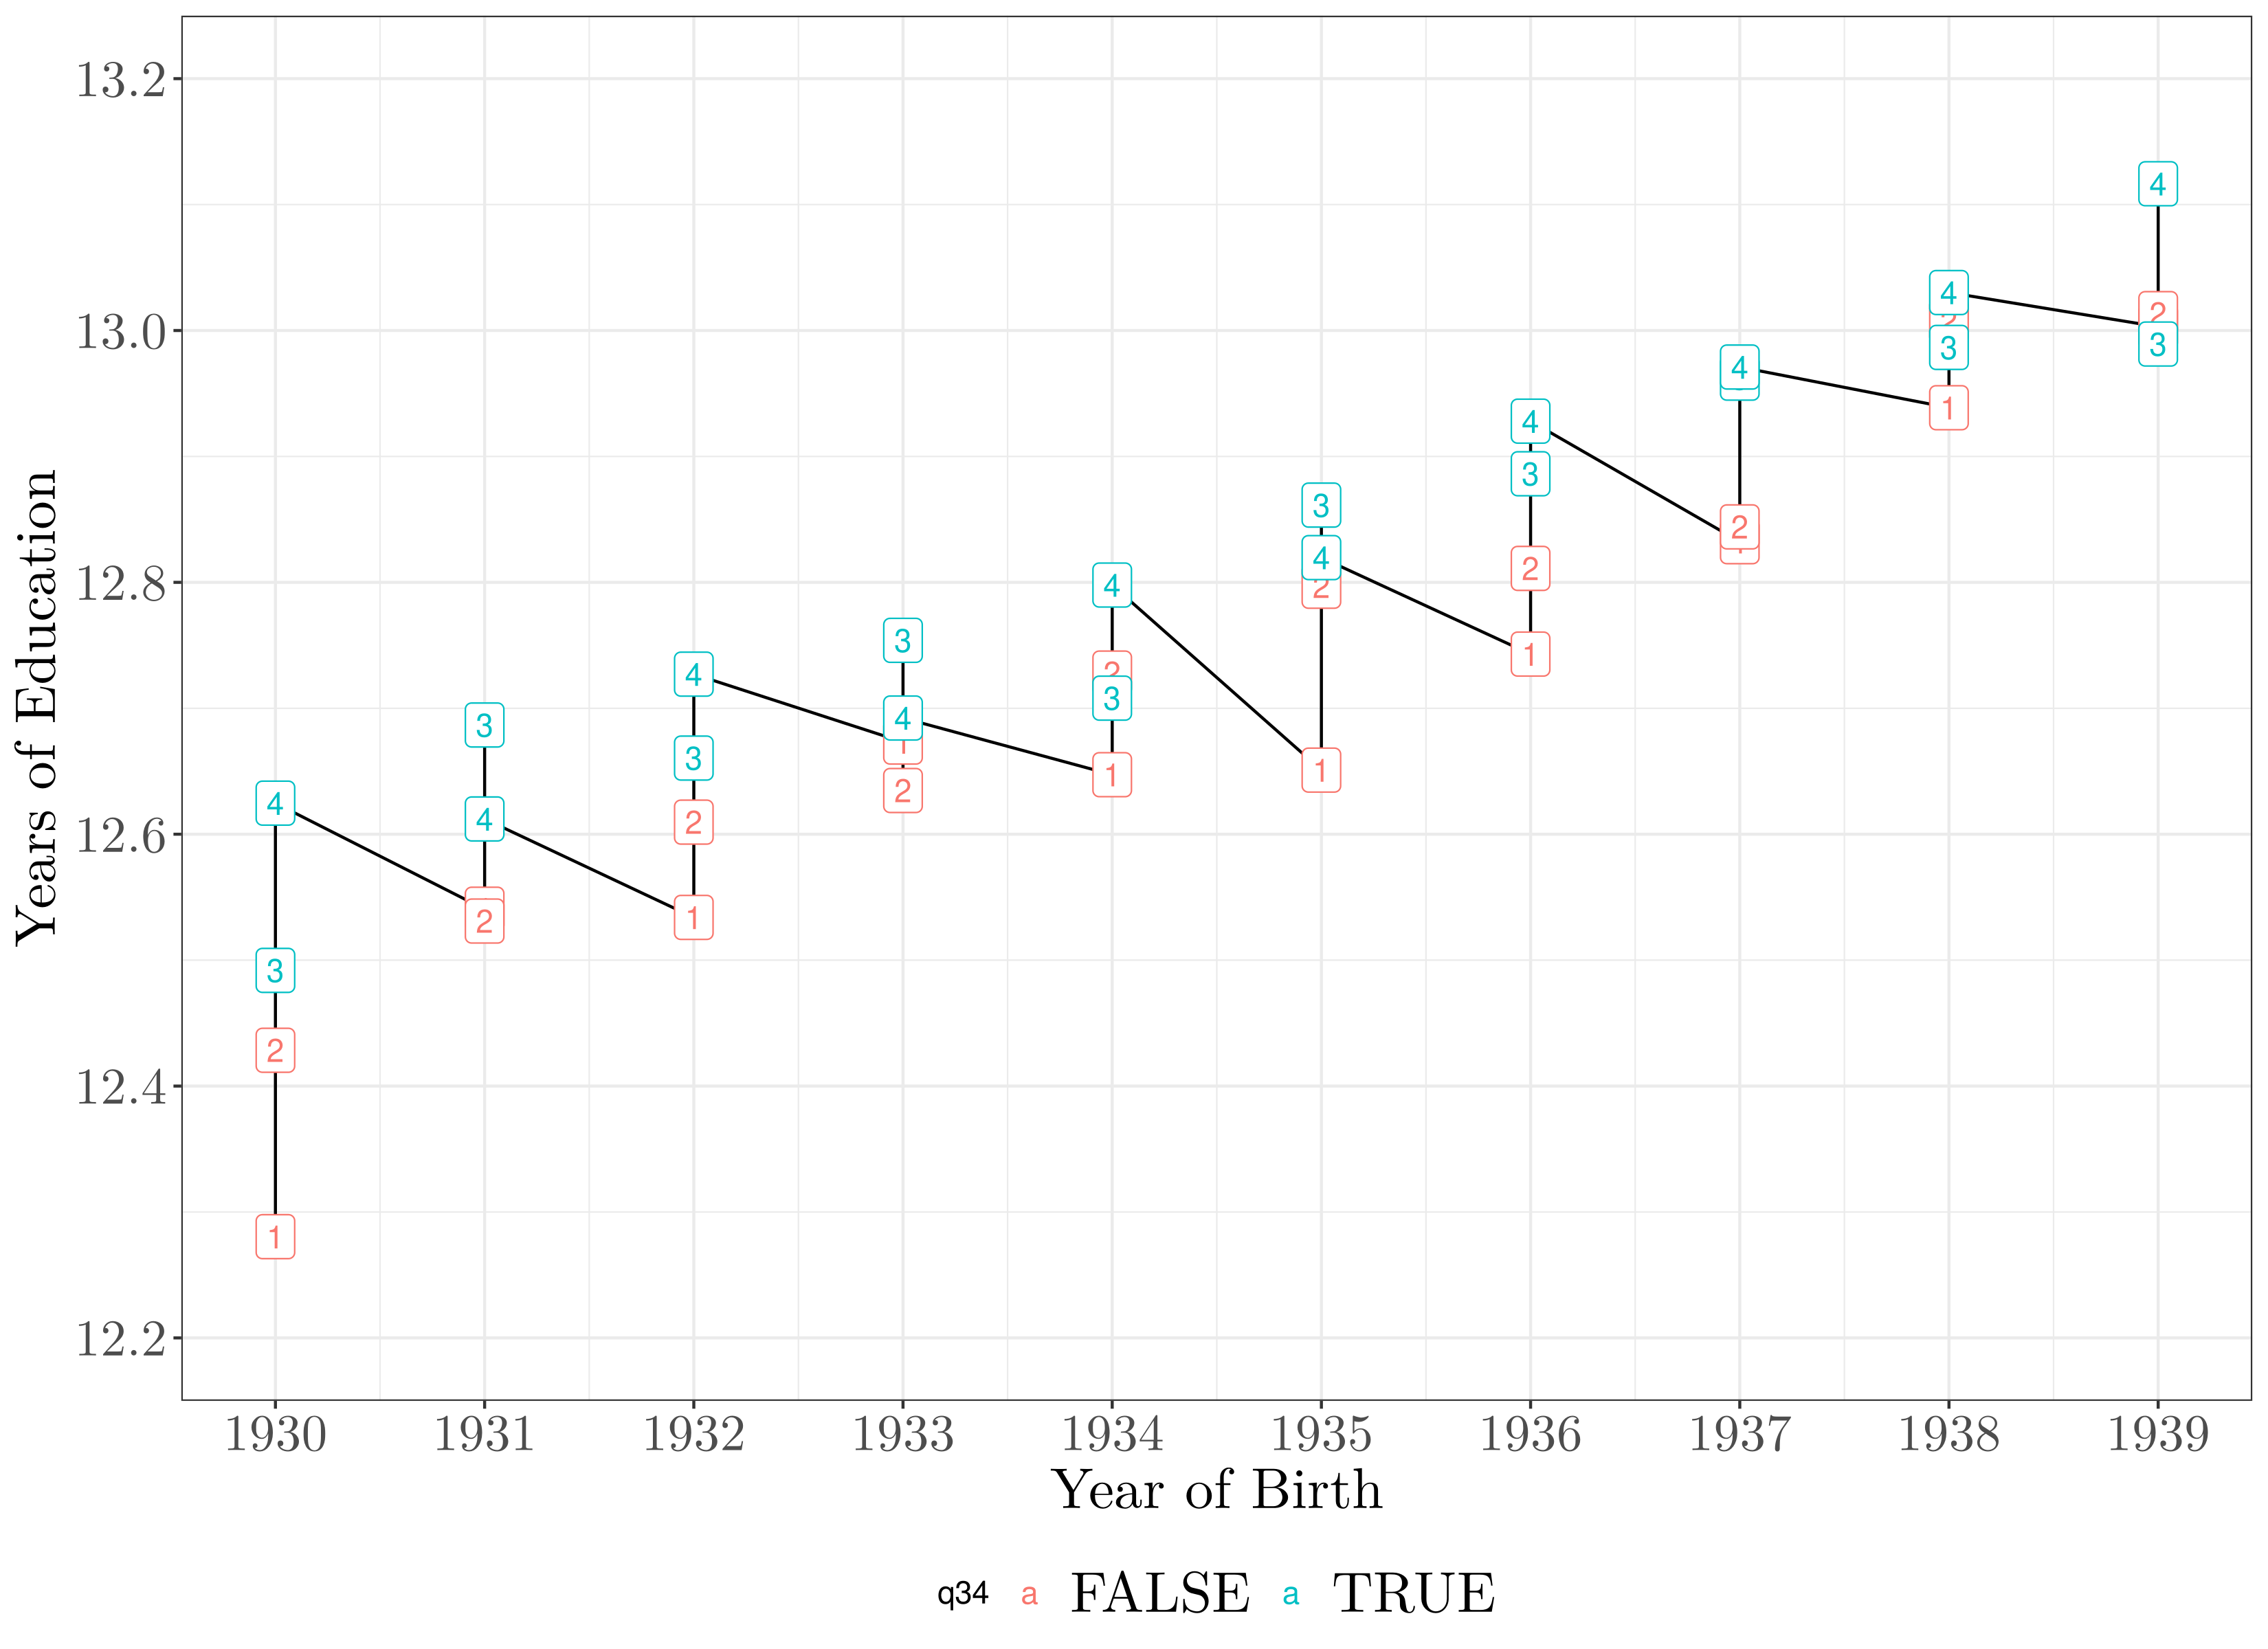
\includegraphics[scale=0.45]{"home/angelo/Documents/Uni/Courses/Advanced Statistics and programming/Assignments/assignment2/Graphics/task3_ivreg_proof.png"}
         \small
         \caption{Displaying association between Quarter of Birth and Years of Education}
\end{figure}

Finally, when considering Figure 2, one can seethat on average, Q4 and Q3 tend to have significantly more years of education than Q1 and Q2 - this might also explain the aforementioend results regarding Q2 difference to Q1 in model (4) in table 7. 


\textbf{IMPORTANT ADD CORRELATION}
Overall, the instrument appears to meet the relevance criterion. 






\begin{table}[!htbp] \centering 
\begin{adjustwidth}{0.cm}{-0cm}
\begin{threeparttable}
\small
\captionsetup{font=small, justification=raggedright,singlelinecheck=false}
\caption{\textsc{First Stage regression output - Relevancy}}
\centering 
  \label{}
\small 
\begin{tabular}{@{\extracolsep{-2pt}}lcccc} 
\\[-5.8ex]\hline 
\hline \\[-1.8ex] 
 & \multicolumn{4}{c}{\textit{Dependent variable:}} \\ 
\cline{2-5} 
\\[-1.8ex] & \multicolumn{4}{c}{educ} \\ 
\\[-1.8ex] & (1) & (2) & (3) & (4)\\ 
\hline \\[-1.8ex] 
 Constant & 12.641$^{***}$ & 15.150$^{***}$ & 12.688$^{***}$ & 15.213$^{***}$ \\ 
  & (0.014) & (0.091) & (0.011) & (0.091) \\ 
  qob & 0.052$^{***}$ & 0.032$^{***}$ &  &  \\ 
  & (0.005) & (0.005) &  &  \\ 
  age &  & $-$0.060$^{***}$ &  & $-$0.060$^{***}$ \\ 
  &  & (0.002) &  & (0.002) \\ 
  married &  & 0.248$^{***}$ &  & 0.248$^{***}$ \\ 
  &  & (0.017) &  & (0.017) \\ 
  qob\_fac2 &  &  & 0.057$^{***}$ & $-$0.004 \\ 
  &  &  & (0.016) & (0.016) \\ 
  qob\_fac3 &  &  & 0.117$^{***}$ & 0.052$^{***}$ \\ 
  &  &  & (0.016) & (0.016) \\ 
  qob\_fac4 &  &  & 0.151$^{***}$ & 0.088$^{***}$ \\ 
  &  &  & (0.016) & (0.016) \\ 
 \hline \\[-1.8ex] 
Observations & 329,509 & 329,509 & 329,509 & 329,509 \\ 
R$^{2}$ & 0.0003 & 0.004 & 0.0003 & 0.004 \\ 
Adjusted R$^{2}$ & 0.0003 & 0.004 & 0.0003 & 0.004 \\ 
Residual Std. Error & 3.281 & 3.275 & 3.281  & 3.275  \\ 
F Statistic & 100.653$^{***}$  & 414.645$^{***}$ & 34.009$^{***}$ & 249.859$^{***}$  \\ 
\hline 
\hline \\[-3.5ex] 
\end{tabular} 
\begin{tablenotes}[para,flushleft]
      \small
      \item\textit{Note:} N = HUUUUGE; so degrees of freedom are not reported for F tests; *** p$<$0.01, ** p$<$0.05, * p$<$0.1
    \end{tablenotes}
\end{threeparttable}
\end{adjustwidth}
%
\end{table}





\textbf{see slide 88; 82}

\begin{enumerate}
   \item here already use the regression outputs from task 4 and also the a correlation table 
   \item add a plot!!!
   \item partial f test for relevance/ strength of the instrument!
   \item summary(rslt2SLS.B, diagnostics = TRUE) --> see the things in tutorial 2 there I descibe all of it; also the slides are relevant
\end{enumerate}

\textbf{A good instrument possesses two specifications: it is clean and it is relevant}



\textbf{HOW DO I CONDUCT THESE TESTS? CAN I CONDUCT THEM ON THE NORMAL 2SLS via OLS or should I better use the IVreg model?}



\subsection{Task 4: Conduct IVreg of the effect of effect of education on log wages, using quarter of birth as the instrument; are robust SE needed?}

\textbf{$NOTE FOR TASK 4: test whether using qob as factor works differently when you only include the 3 dummies for it instaead of qob_fac$}



For the purpose of this analysis, it is assumed that the control variables are all exogenoeus. Table 8 reports the corresponding outputs; model (1) and (3) consider qob as a numeric variable and model (2) and (4) consider it as a categorical variable. It may be noted that qob should be interpreted as a categorical variable to be precise.
Models (5) and (6) consider an additional instrument (discussed in part 5).
The control variables chosen are SMSA and whether married or not. Married was included because the proportion of married men tends to be higher for higher educated men, suggesting more education but also more income. Moreover, SMSA indicates whether a person lives in a rural or urban surrounding; people in urban areas may have better access to education and better work opportunities.
Considering model (3) and (4), the causal variable education is significant (model 3: $\hat{\beta}$ = 0.099, $p$ $<$ 0.01; model 4: $\hat{\beta}$ = 0.103, $p$ $<$ 0.01). Considering for instance qob as a categorical IV, (model 4) we can see that if education increases by one year wage increases by 10.2\%. Moving to model (5 / 6) we can also see that the choice between qob as numeric or category seems to have little effect on the general statement.
COnsidering model (6), which contains SMSA and married as exogenous controls, the direction and magnitude, in addition to reported standard errors, for years of education do not change considerably when compared to model (4) (both qob as factor IV) ($\hat{\beta}$ = 0.100, $p$ $<$ 0.01). Meaning, that an increase by one year in years of education is associated with a 10\% higher wage. ALso the control variables are significant which are both categoricals (SMSA comparison category is rural; married comparison category is not maried) (SMSA: $\hat{\beta}$ = -0.148, $p$ $<$ 0.01; married: $\hat{\beta}$ = -0.255, $p$ $<$ 0.01); However, due to them being controls, we refrain from interpreting them here as we did with education. 

TO DO: Include PLOT AND BPAGAN TEST INFERENCE HERE
 \textbf{ROBUST STANDARD ERRORS!!!}
 
%Column (1): this model explains 9.8% of the variation in the outcome variable. An additional year of
%education is associated with an increase in the log wage by 9.9%. This effect is highly statistically significant
%on any conventional levels of significance. The constant is also highly significant.
%Column (2): when qob is used as a factor, this variable explains 9.4% of the variation in the outcome
%variable. Now, an additional year of education is associated with a highly significant increase in the log wage
%by 10.3%. The constant is again highly significant and is it important to note that the intercept effect of Q1
%is included in the constant.
%Column (3): When adding yob as a control variable, an additional year of education is associated with an
%increase in the log wage by 10.2%. This effect is highly significant. This model explains 9.5% of the variation
%in the outcome variable
%Column (4): When adding yob as a control variable, an additional year of education is associated with an
%increase in the log wage by 10.5%. This effect is highly significant. This model explains 9.1% of the variation
%in the outcome variable.

%In the IV regression without control variables the education coefficient is statistically significant ($\beta$ = 0.103, p $<$ 0.01). In the IV regression with control variables the education coefficient is also statistically significant ($\beta$ = 0.102, p $<$ 0.01). When the education goes up by one year, the wages will increase by approximately 10.2 percent. Also the married control variable is statistically significant ($\beta$ = 0.248, p $<$ 0.01). When a person is married their wage increases by approximately 24.8 percent. For the 2SLS regression with over identification, 'educ' is statistically significant ($\beta$ = 0.231, p $<$ 0.01). This result can be interpreted as when an additional year of education is followed the wage increases by approximately 23.1 percent. This is more than twice as high as in the IV regression before. The control variable married is also statistically significant in this model ($\beta$ = 0.218, p $<$ 0.01). The difference between the last two models might be caused by endogeneity of the instruments used. In figure 5 the summary statistics are given of the last regression. When looking at the Sargan test statistic the null hypothesis of no violation of exogeneity by over-identification is rejected. Lastly, I checked whether using robust standard errors affected my results. The results from the regression using white's standard errors are found in appendix E. Using robust standard errors had no affect on the models.


% Table created by stargazer v.5.2.3 by Marek Hlavac, Social Policy Institute. E-mail: marek.hlavac at gmail.com
% Date and time: Thu, Sep 29, 2022 - 12:17:17
\begin{table}[!htbp] \centering 
\begin{adjustwidth}{0.cm}{-0cm}
\begin{threeparttable}
\small
\captionsetup{font=small, justification=raggedright,singlelinecheck=false}
\caption{\textsc{IV regression output}}
\centering 
  \label{}
\small 
\begin{tabular}{@{\extracolsep{-5pt}}lcccccc} 
\\[-5.8ex]\hline 
\hline \\[-1.8ex] 
 & \multicolumn{6}{c}{\textit{Dependent variable:}} \\ 
\cline{2-7} 
\\[-1.8ex] & \multicolumn{6}{c}{lnwage} \\ 
\\[-1.8ex] & (1) & (2) & (3) & (4) & (5) & (6)\\ 
\hline \\[-1.8ex] 
 Constant & 4.633$^{***}$ & 4.590$^{***}$ & 4.461$^{***}$ & 4.425$^{***}$ & 5.514$^{***}$ & 5.511$^{***}$ \\ 
  & (0.250) & (0.249) & (0.249) & (0.248) & (0.076) & (0.076) \\ 
  educ & 0.099$^{***}$ & 0.103$^{***}$ & 0.098$^{***}$ & 0.100$^{***}$ & 0.015$^{**}$ & 0.015$^{**}$ \\ 
  & (0.020) & (0.020) & (0.020) & (0.019) & (0.006) & (0.006) \\ 
  SMSA &  &  & $-$0.151$^{***}$ & $-$0.148$^{***}$ & $-$0.243$^{***}$ & $-$0.243$^{***}$ \\ 
  &  &  & (0.022) & (0.022) & (0.007) & (0.007) \\ 
  married &  &  & 0.256$^{***}$ & 0.255$^{***}$ & 0.280$^{***}$ & 0.280$^{***}$ \\ 
  &  &  & (0.006) & (0.006) & (0.004) & (0.004) \\ 
 \hline \\[-1.8ex] 
Observations & 329,509 & 329,509 & 329,509 & 329,509 & 329,509 & 329,509 \\ 
R$^{2}$ & 0.098 & 0.094 & 0.124 & 0.120 & 0.082 & 0.083 \\ 
Adjusted R$^{2}$ & 0.098 & 0.094 & 0.124 & 0.120 & 0.082 & 0.083 \\ 
Residual Std. Error & 0.645  & 0.646  & 0.635  & 0.637 & 0.650 & 0.650  \\ 
\hline 
\hline \\[-3.5ex] 
\end{tabular} 
\begin{tablenotes}[para,flushleft]
      \small
      \item\textit{Note:} N = HUUUUGE; so degrees of freedom are not reported for F tests. *** p$<$0.01, ** p$<$0.05, * p$<$0.1.
    \end{tablenotes}
\end{threeparttable}
\end{adjustwidth}
%
\end{table}










\begin{enumerate}
   \item IT IS VERY IMPORTANT TO BUILD A QUICK THEORY AND ALSO EXPLAIN WHY THE CONTROL VARIABLES ARE EXOGENOEUS; SO WHY THERE CONTROLS ARE RELEVANT!!!!!
   \item also look at the examples in those links how they didd this !
\end{enumerate}








%$https://rpubs.com/wsundstrom/t_ivreg"
%https://stats.stackexchange.com/questions/56722/where-do-i-put-the-control-variables-in-2sls
\textbf{IMPORTANT: IF YOU INCLUDE CONTROL VARIABLES YOU NEED TO ARGUE WHY THEY ARE EXOGENEOUS OR NOT AS THAT THEY ARE INCLDUED INTO THE EQUATION}
SLIDE 99
IMPORTANT: USE slide 88 as an argument

\textbf{IMPORTANT: WHEN YOU SAY HOW CONTROL VARIABLES IMPACT THE INDEPENDENT VARIABLE SAY THE INCLUSION OF THE CONTROL VARIABLES ICNREASE IT INTO A CERTAIN DIRECTIOn; SO DEPEDNING ON THE INSTRUMENT VS NORMAL OLS, the variable was biased eg downwards or upwards}

\subsection{5 -- }

% Table created by stargazer v.5.2.3 by Marek Hlavac, Social Policy Institute. E-mail: marek.hlavac at gmail.com
% Date and time: Thu, Sep 29, 2022 - 17:18:36
\begin{table}[!htbp] \centering 
\begin{adjustwidth}{0.cm}{-0cm}
\begin{threeparttable}
\small
\captionsetup{font=small, justification=raggedright,singlelinecheck=false}
\caption{\textsc{IV regression output}}
\centering 
  \label{}
\small 
\begin{tabular}{@{\extracolsep{-5pt}}lcccccc} 
\\[-5.8ex]\hline 
\hline \\[-1.8ex] 
 & \multicolumn{6}{c}{\textit{Dependent variable:}} \\ 
\cline{2-7} 
\\[-1.8ex] & \multicolumn{6}{c}{lnwage} \\ 
\\[-1.8ex] & OLS (1) & OLS (2) & HandIVREG(3) & HandIVREG(4) & HandIVREG(5) & HandIVREG(6)\\ 
\hline \\[-1.8ex] 
 Constant & 4.995$^{***}$ & 4.847$^{***}$ & 4.633$^{***}$ & 4.461$^{***}$ & 4.590$^{***}$ & 4.425$^{***}$ \\ 
  & (0.004) & (0.005) & (0.263) & (0.260) & (0.262) & (0.259) \\ 
  educ & 0.071$^{***}$ & 0.067$^{***}$ &  &  &  &  \\ 
  & (0.0003) & (0.0003) &  &  &  &  \\ 
  SMSA &  & $-$0.185$^{***}$ &  & $-$0.151$^{***}$ &  & $-$0.148$^{***}$ \\ 
  &  & (0.003) &  & (0.023) &  & (0.023) \\ 
  married &  & 0.265$^{***}$ &  & 0.256$^{***}$ &  & 0.255$^{***}$ \\ 
  &  & (0.003) &  & (0.007) &  & (0.007) \\ 
  educ.hat &  &  & 0.099$^{***}$ & 0.098$^{***}$ & 0.103$^{***}$ & 0.100$^{***}$ \\ 
  &  &  & (0.021) & (0.020) & (0.020) & (0.020) \\ 
 \hline \\[-1.8ex] 
Observations & 329,509 & 329,509 & 329,509 & 329,509 & 329,509 & 329,509 \\ 
R$^{2}$ & 0.117 & 0.145 & 0.0001 & 0.041 & 0.0001 & 0.041 \\ 
Adjusted R$^{2}$ & 0.117 & 0.145 & 0.0001 & 0.041 & 0.0001 & 0.041 \\ 
Residual Std. Error & 0.638 & 0.628 & 0.679 & 0.665  & 0.679& 0.665  \\ 
F Statistic & 43,782.560$^{***}$ & 18,646.640$^{***}$  & 23.145$^{***}$  & 4,738.984$^{***}$ & 25.088$^{***}$ & 4,739.535$^{***}$ \\ 
\hline 
\hline \\[-3.5ex] 
\end{tabular} 
\begin{tablenotes}[para,flushleft]
      \small
      \item\textit{Note:} ALL ARE IV REGRESSION OUTPUTS!!! tests. *** p$<$0.01, ** p$<$0.05, * p$<$0.1.
    \end{tablenotes}
\end{threeparttable}
\end{adjustwidth}
%
\end{table}
Note: this question was not particularly precise wrt. whether to run a manual 2SLS or just normal OLS.

Model (1) and (2) in Table 9 report the OLS regressions of lnwage on the endogeneous education with and without covariates. Models (3) and (4) report the manual 2SLS for quarter of birth as a numeric. Models (5) and (6) report quarter of birth as a factor. 

\indent Considering model (2), standard OLS with covaraiates, the overall effect of education on is significantly positie ($\hat{\beta}$ = 0.067, $p$ $<$ 0.01), which does not deviate drasically from its (assumed) exogeneous counterpart in the other models in Table 8 (and 9). However, we can observe a considerably lower standard error for the years of education coefficient in model (2) when compared to Table 8 models 1 through 6.

\indent Moving on now to the manual 2SLS, as expected, the reported coefficients in models 3 thorugh 6 in Table 9 correspond exactly with those reported in Table 8 (models 1 through 4). However, the manual 2SLS does not correct for the fact that years of education (hat) originates as a predicted outcome of the first stage. Thus, the standard errors differ slightly.
\indent COnsidering how which model to prefer, OLS vs model of methods or IVREG, the Hausman's ${\chi}^2$ can be used to assess which estimator is to be preferred. These are output from the $summary(IVREG_model, diagnostics = TRUE)$ in R, together with a test for weak instruments and, in case of overidentification, the Sargan-Hansen ${\chi}^2$ over-identification test. To keep it short, two models are considered fro demonstrative purposes: 1) Table 8 model (3) where qob is a numeric varaible (so no overidentification), and 2) Table 8 model (5) is considered where $yob$ (year of birth) was added as an instrument to demonstrate over identification. Please note that thechically, the inclusion of qob as a factor implies overidentification of the first stage; this will be ignored in this question.

\indent Considering Table 10, the weak instruments test, which is just a partial F-test on the first stage of 2SLS, reports significant F statistics for both models (model 3: $F Statistic$ = 100.159, $p$ $<$ 0.01; model 5:$F Statistic$ = 557.21, $p$ $<$ 0.01), suggesting that the relevance criterion is fulfilled. Moving to the Wu-Hausman test however, the models differ. Model (3) (qob numeric model) reports and insignificant test statistic (${\chi}^2$ = 2.477, $p$ = 0.116), suggesting a preference for the OLS estimator. Contrarily, Model (5) reports a significant test statistic (${\chi}^2$ = 82.16), suggesting that the usage of model of methods (2SLS) is preferred over OLS in this case.\footnote{Please note that I included this example on purpose} Finally, considering the question of overidentification, this is not applicable to model (3), when considering qob as a numeric; it would, however, be relevant if we considered qob as a factor. Model (5), on the other hand, contains a second instrument, year of birth, as a demonstrative example. As can be seen in Table 10, the Sargan-Hansen ${\chi}^2$ test of overidentification reports a significant test statistic (${\chi}^2$ = 18.84, $p$ $<$ 0.01). Rejecting the null hypothesis implies that indepedence of the instruments of the residuals cannot be assumed. Thus, the instruments themselfes are assumed to be endogeneous themselfes and overidentification poses a problem for model (5). It may be interesting to note that if we considered qob as a factor, this test statistic would be insignificant, suggesting that the qob as a factor is exogenoeus and, thus, overidentification is no problem. 



                    df1    df2 statistic p-value    
Weak instruments      1 329505   100.159  <2e-16 ***
Wu-Hausman            1 329504     2.477   0.116    
Sargan                0     NA        NA      NA    

Diagnostic tests:
                    df1    df2 statistic  p-value    
Weak instruments      2 329504    557.21  < 2e-16 ***
Wu-Hausman            1 329504     82.16  < 2e-16 ***
Sargan                1     NA     18.84 1.42e-05 ***



\subsection{6 -- }
\textbf{Relevantce: Contrarily, this assumption can be tested: it states that the instrument used for the "to be instrumentalize" variable is strong, meaning that there is a relevant correlation between the instrument and the independent variables. Note: a correlation between the instrument adn the independent variables beyond the baised variable is welcome. It only becomes a problem when the instrument and the dependent varaible are related; btu there will always be some correlation in that regard. To this end, an anova is run on the two stage model in order to conduct the F test, which helps with multiple outputs: Wu-Hausman, Sargan, and F test (the former two are only relevant if the model is overidentified by the instrument)}

Elaborate on possible causes of concern that could render your instrumen-
tal variable identification strategy invalid. Base your argumentation on
the required assumptions of instrumental variables as taught in the lecture.
An arbitrarily made-up example would be: “Birthdays in the US have
been recorded with a varying delay between 1 and 6 months. Hence, the
measurement of school years for dropout students could be inaccurate.”



There are multiple ways which could invalidate the ninstrumental variable identification strategy invalid. 1) the instrument may not be relevant for the endogeneous variable; it is notable that correaltion does not necessarily guarantee relevance. Thus, it might actually be the case that qob is just not a relvant instrument and that the correlation is not strong enough. 2) The (supposed) variable years of education is actually not endogeneous; remember that this is mostly based on theory and not on tests.
However, the most interesting point to discuss is considers 3) the cleanliness of the instrument. This would mean, that qob does not only have an effect on lnwage through the edogeneous variable alone, but rather is a confounder itself, thus, having an impact on lnwage. 
4) the instrument is endogeneous itself; such as measuremtn errors or it may be realted to further backdoor paths such as socioeconomic status. 

%Although it seems reasonable to think that qob has an impact on education exclusively because of compulsory
%schooling, we will examine the validity of this instrument. In order to be valid, an instrument must fulfil the
%following two assumptions:
%• relevance: the IV is preferably strongly correlated with the explanatory variables (i.e. cov(Z, X) 6= 0).
%• exogeneity: the IV is uncorrelated with the disturbances in the regression model, meaning that qob
%only affects the lnwage through educ (i.e. cov(Z, u) = 0).
%As relevance was discussed in chapter 2.3 of this assignment, we will examine the exogeneity assumption.
%Age may play a role in academic performance. Indeed, it could be that students born in Q1 start school at
%an older age and are, thus, more mature and perform better in school. From another angle, students born in
%Q1 benefit from less time in school (for compulsory education). This would then bias the result and make the
%IV invalid.
%It is also possible that qob is related to the socioeconomic status of children’s parents. Indeed, there could
%be a connection between quarter of birth and education. For example, we could observe more unwanted
%pregnancies in a specific quarter and this would bias the result and make the IV invalid.


CLeanliness; Endogeneity of independent; Relevance
--> Cleanliness 


\begin{enumerate}
   \item not clean insutruments! this would lead to violation of mean independence
   \item weak insturments leads to mean indepdence violation as well becasue the indstruments simply do not work as they should 
   \item google some stuff and see internet
\end{enumerate}



reasons: not clear instrument (or not clean) (make a plot; or if the instrument is not relevant or weak)

%$https://rpubs.com/wsundstrom/t_ivreg"
%https://stats.stackexchange.com/questions/56722/where-do-i-put-the-control-variables-in-2sls --> a possible plot

%https://www.econometrics-with-r.org/12-3-civ.html
% Plot https://www.statisticshowto.com/instrumental-variable/












\section{Bibliography}






\section{Appendix}


% Table created by stargazer v.5.2.3 by Marek Hlavac, Social Policy Institute. E-mail: marek.hlavac at gmail.com
% Date and time: Fri, Sep 23, 2022 - 20:47:48
\begin{table}[!htbp] 
\begin{adjustwidth}{-0cm}{-0cm}
\begin{threeparttable}
\small
\captionsetup{font=small, justification=raggedright,singlelinecheck=false}
  \caption{Descriptive Statistics of ECIC; With Children} 
  \label{} 
\begin{tabular}{@{\extracolsep{5pt}}lccccccc} 
\\[-1.8ex]\hline 
\hline \\[-1.8ex] 
Statistic & \multicolumn{1}{c}{Mean} & \multicolumn{1}{c}{St. Dev.} & \multicolumn{1}{c}{Min} & \multicolumn{1}{c}{Pctl(25)} & \multicolumn{1}{c}{Median} & \multicolumn{1}{c}{Pctl(75)} & \multicolumn{1}{c}{Max} \\ 
\hline \\[-1.8ex] 
Family Income & 12,750.390 & 15,739.050 & 0.000 & 4,652.465 & 8,425.197 & 15,218.720 & 410,507.600 \\ 
Earnings & 7,909.934 & 14,956.930 & 0.000 & 0.000 & 1,110.727 & 11,107.270 & 366,095.500 \\ 
Age & 32.717 & 8.630 & 20 & 25 & 32 & 39 & 54 \\ 
Education & 9.001 & 2.408 & 0 & 7 & 10 & 11 & 11 \\ 
Education Years & 4.840 & 5.872 & 0.000 & 0.071 & 3.761 & 7.070 & 102.958 \\ 
Unearned Income & 2.097 & 1.209 & 1 & 1 & 2 & 3 & 9 \\ 
Count Children & 0.466 & 0.499 & 0 & 0 & 0 & 1 & 1 \\ 
\hline \\[-1.8ex] 
\end{tabular} 
\begin{tablenotes}[para,flushleft]
      \small
      \item\textit{Notes:} N = 7819
    \end{tablenotes}
\end{threeparttable}
\end{adjustwidth}
\end{table} 




% Table created by stargazer v.5.2.3 by Marek Hlavac, Social Policy Institute. E-mail: marek.hlavac at gmail.com
% Date and time: Fri, Sep 23, 2022 - 20:47:48
\begin{table}[!htbp] 
\begin{adjustwidth}{-0cm}{-0cm}
\begin{threeparttable}
\small
\captionsetup{font=small, justification=raggedright,singlelinecheck=false}
  \caption{Descriptive Statistics of ECIC; Without Children} 
  \label{} 
\begin{tabular}{@{\extracolsep{5pt}}lccccccc} 
\\[-1.8ex]\hline 
\hline \\[-1.8ex] 
Statistic & \multicolumn{1}{c}{Mean} & \multicolumn{1}{c}{St. Dev.} & \multicolumn{1}{c}{Min} & \multicolumn{1}{c}{Pctl(25)} & \multicolumn{1}{c}{Median} & \multicolumn{1}{c}{Pctl(75)} & \multicolumn{1}{c}{Max} \\ 
\hline \\[-1.8ex] 
Family Income & 18,559.860 & 23,041.780 & 0.000 & 5,793.092 & 11,912.950 & 24,391.010 & 575,616.800 \\ 
Earnings & 13,760.260 & 21,301.400 & 0.000 & 0.000 & 7,664.014 & 19,447.610 & 537,880.600 \\ 
Age & 38.498 & 11.046 & 20 & 28 & 40 & 49 & 54 \\ 
Education & 8.549 & 2.889 & 0 & 7 & 10 & 11 & 11 \\ 
Education Years & 4.800 & 8.496 & 0.000 & 0.000 & 1.248 & 6.528 & 134.058 \\ 
Unearned Income & 0.000 & 0.000 & 0 & 0 & 0 & 0 & 0 \\ 
Count Children & 0.574 & 0.494 & 0 & 0 & 1 & 1 & 1 \\ 
\hline \\[-1.8ex] 
\end{tabular} 
\begin{tablenotes}[para,flushleft]
      \small
      \item\textit{Notes:} N = 5927
    \end{tablenotes}
\end{threeparttable}
\end{adjustwidth}
\end{table}


% Table created by stargazer v.5.2.3 by Marek Hlavac, Social Policy Institute. E-mail: marek.hlavac at gmail.com
% Date and time: Wed, Sep 14, 2022 - 15:53:27
\begin{table}[!htbp] \centering 
\begin{adjustwidth}{0.cm}{-0cm}
\begin{threeparttable}
\small
\captionsetup{font=small, justification=raggedright,singlelinecheck=false}
\caption{\textsc{Non-Robust Regression Results Part 3}}
\centering 
  \label{}
\small 
\begin{tabular}{@{\extracolsep{-2pt}}lcccccc} 
\\[-5.8ex]\hline 
\hline \\[-1.8ex] 
 & \multicolumn{6}{c}{\textit{Dependent variable:}} \\ 
\cline{2-7} 
\\[-1.8ex] & \multicolumn{2}{c}{earn} & \multicolumn{2}{c}{finc} & \multicolumn{2}{c}{work} \\ 
\\[-1.8ex] & (1) & (2) & (3) & (4) & (5) & (6)\\ 
\hline \\[-1.8ex] 
 Constant & 14,899.900$^{***}$ & 12,958.640$^{***}$ & 20,099.430$^{***}$ & 16,218.430$^{***}$ & 0.582$^{***}$ & 0.532$^{***}$ \\ 
  & (828.375) & (1,550.012) & (886.522) & (1,655.347) & (0.023) & (0.043) \\ 
  has\_children1 & $-$8,596.327$^{***}$ & $-$8,394.973$^{***}$ & $-$8,929.330$^{***}$ & $-$8,269.567$^{***}$ & $-$0.159$^{***}$ & $-$0.150$^{***}$ \\ 
  & (1,093.444) & (1,096.506) & (1,170.197) & (1,171.022) & (0.030) & (0.030) \\ 
  dperiod & $-$695.997 & $-$536.491 & $-$940.239$^{*}$ & $-$515.553 & $-$0.005 & $-$0.024$^{*}$ \\ 
  & (485.413) & (500.046) & (519.486) & (534.028) & (0.013) & (0.014) \\ 
  age &  & 22.555 &  & 78.717$^{***}$ &  & 0.002$^{***}$ \\ 
  &  & (15.922) &  & (17.004) &  & (0.0004) \\ 
  urate &  & 133.948 &  & 372.861$^{***}$ &  & $-$0.018$^{***}$ \\ 
  &  & (114.614) &  & (122.403) &  & (0.003) \\ 
  ed &  & 66.337 &  & $-$125.305$^{**}$ &  & 0.017$^{***}$ \\ 
  &  & (59.579) &  & (63.628) &  & (0.002) \\ 
  nonwhite1 &  & $-$1,255.622$^{***}$ &  & $-$2,438.387$^{***}$ &  & $-$0.043$^{***}$ \\ 
  &  & (326.237) &  & (348.408) &  & (0.009) \\ 
  has\_children1:dperiod & 1,682.810$^{***}$ & 1,722.360$^{***}$ & 1,911.035$^{***}$ & 2,006.060$^{***}$ & 0.031$^{*}$ & 0.033$^{*}$ \\ 
  & (642.099) & (641.893) & (687.171) & (685.515) & (0.018) & (0.018) \\ 
 \hline \\[-1.8ex] 
R$^{2}$ & 0.026 & 0.027 & 0.022 & 0.028 & 0.012 & 0.027 \\ 
Adjusted R$^{2}$ & 0.026 & 0.027 & 0.022 & 0.027 & 0.012 & 0.026 \\ 
Residual Std. Error & 17,965.670 & 17,956.450  & 19,226.750  & 19,176.730 & 0.497  & 0.493  \\ 
F Statistic & 121.691$^{***}$ & 54.794$^{***}$ & 105.245$^{***}$ & 56.166$^{***}$  & 54.906$^{***}$  & 54.374$^{***}$  \\ 
\hline 
\hline \\[-3.5ex] 
\end{tabular} 
\begin{tablenotes}[para,flushleft]
      \small
      \item\textit{Note:} N = 13746. Non Robust Standard Errors applied. "White" is reference category for "non-White" categorical variable.
    \end{tablenotes}
\end{threeparttable}
\end{adjustwidth}
%
\end{table}

\begin{landscape}
% Table created by stargazer v.5.2.3 by Marek Hlavac, Social Policy Institute. E-mail: marek.hlavac at gmail.com
% Date and time: Wed, Sep 28, 2022 - 18:35:54
\begin{table}[!htbp] \centering 
\begin{adjustwidth}{1.25cm}{-0cm}
\begin{threeparttable}
\small
\captionsetup{font=small, justification=raggedright,singlelinecheck=false}
\caption{\textsc{Non-Robust Regression Results Part 3}}
\centering 
  \label{}
\small 
\begin{tabular}{@{\extracolsep{-2pt}}lccccccccc} 
\\[-5.8ex]\hline 
\hline \\[-1.8ex] 
 & \multicolumn{9}{c}{\textit{Dependent variable:}} \\ 
\cline{2-10} 
\\[-1.8ex] & \multicolumn{3}{c}{earn} & \multicolumn{3}{c}{finc} & \multicolumn{3}{c}{work} \\ 
\\[-1.8ex] & Basic(1) & White(2) & Cluster(3) & Basic(4) & White(5) & Cluster(6) & Basic(7) & White(8) & Cluster(9)\\ 
\hline \\[-1.8ex] 
 has\_children1 & $-$8,394.973$^{***}$ & $-$8,394.973$^{***}$ & $-$8,394.973$^{***}$ & $-$8,269.567$^{***}$ & $-$8,269.567$^{***}$ & $-$8,269.567$^{***}$ & $-$0.150$^{***}$ & $-$0.150$^{***}$ & $-$0.150$^{***}$ \\ 
  & (1,096.506) & (1,056.274) & (1,057.069) & (1,171.022) & (1,146.704) & (1,147.577) & (0.030) & (0.030) & (0.030) \\ 
  & & & & & & & & & \\ 
 dperiod & $-$536.491 & $-$536.491 & $-$536.491 & $-$515.553 & $-$515.553 & $-$515.553 & $-$0.024$^{*}$ & $-$0.024$^{*}$ & $-$0.024$^{*}$ \\ 
  & (500.046) & (564.674) & (565.075) & (534.028) & (618.997) & (619.444) & (0.014) & (0.014) & (0.014) \\ 
  & & & & & & & & & \\ 
 age & 22.555 & 22.555 & 22.555 & 78.717$^{***}$ & 78.717$^{***}$ & 78.717$^{***}$ & 0.002$^{***}$ & 0.002$^{***}$ & 0.002$^{***}$ \\ 
  & (15.922) & (19.063) & (19.077) & (17.004) & (20.183) & (20.198) & (0.0004) & (0.0004) & (0.0004) \\ 
  & & & & & & & & & \\ 
 urate & 133.948 & 133.948 & 133.948 & 372.861$^{***}$ & 372.861$^{***}$ & 372.861$^{***}$ & $-$0.018$^{***}$ & $-$0.018$^{***}$ & $-$0.018$^{***}$ \\ 
  & (114.614) & (114.009) & (114.096) & (122.403) & (123.441) & (123.537) & (0.003) & (0.003) & (0.003) \\ 
  & & & & & & & & & \\ 
 ed & 66.337 & 66.337 & 66.337 & $-$125.305$^{**}$ & $-$125.305$^{*}$ & $-$125.305$^{*}$ & 0.017$^{***}$ & 0.017$^{***}$ & 0.017$^{***}$ \\ 
  & (59.579) & (59.876) & (59.937) & (63.628) & (67.467) & (67.538) & (0.002) & (0.002) & (0.002) \\ 
  & & & & & & & & & \\ 
 nonwhite1 & $-$1,255.622$^{***}$ & $-$1,255.622$^{***}$ & $-$1,255.622$^{***}$ & $-$2,438.387$^{***}$ & $-$2,438.387$^{***}$ & $-$2,438.387$^{***}$ & $-$0.043$^{***}$ & $-$0.043$^{***}$ & $-$0.043$^{***}$ \\ 
  & (326.237) & (341.701) & (341.929) & (348.408) & (368.776) & (369.027) & (0.009) & (0.009) & (0.009) \\ 
  & & & & & & & & & \\ 
 has\_children1:dperiod & 1,722.360$^{***}$ & 1,722.360$^{***}$ & 1,722.360$^{***}$ & 2,006.060$^{***}$ & 2,006.060$^{***}$ & 2,006.060$^{***}$ & 0.033$^{*}$ & 0.033$^{*}$ & 0.033$^{*}$ \\ 
  & (641.893) & (647.317) & (647.764) & (685.515) & (698.628) & (699.118) & (0.018) & (0.018) & (0.018) \\ 
  & & & & & & & & & \\ 
 Constant & 12,958.640$^{***}$ & 12,958.640$^{***}$ & 12,958.640$^{***}$ & 16,218.430$^{***}$ & 16,218.430$^{***}$ & 16,218.430$^{***}$ & 0.532$^{***}$ & 0.532$^{***}$ & 0.532$^{***}$ \\ 
  & (1,550.012) & (1,622.488) & (1,623.778) & (1,655.347) & (1,771.017) & (1,772.450) & (0.043) & (0.042) & (0.042) \\ 
  & & & & & & & & & \\ 
\hline \\[-1.8ex] 
Observations & 13,746 & 13,746 & 13,746 & 13,746 & 13,746 & 13,746 & 13,746 & 13,746 & 13,746 \\ 
R$^{2}$ & 0.027 & 0.027 & 0.027 & 0.028 & 0.028 & 0.028 & 0.027 & 0.027 & 0.027 \\ 
Adjusted R$^{2}$ & 0.027 & 0.027 & 0.027 & 0.027 & 0.027 & 0.027 & 0.026 & 0.026 & 0.026 \\ 
Residual Std. Error  & 17,956.450 & 17,956.450 & 17,956.450 & 19,176.730 & 19,176.730 & 19,176.730 & 0.493 & 0.493 & 0.493 \\ 
F Statistic  & 54.794$^{***}$ & 54.794$^{***}$ & 54.794$^{***}$ & 56.166$^{***}$ & 56.166$^{***}$ & 56.166$^{***}$ & 54.374$^{***}$ & 54.374$^{***}$ & 54.374$^{***}$ \\ 
\hline 
\hline \\[-3.5ex] 
\end{tabular} 
\begin{tablenotes}[para,flushleft]
      \small
      \item\textit{Note:} N = 13746. Robust Standard Errors applied. "White" is reference category for "non-White" categorical variable. *** p$<$0.01, ** p$<$0.05, * p$<$0.1.
    \end{tablenotes}
\end{threeparttable}
\end{adjustwidth}
%
\end{table}

\end{landscape}


\section{Code}



% Table created by stargazer v.5.2.3 by Marek Hlavac, Social Policy Institute. E-mail: marek.hlavac at gmail.com
% Date and time: Sun, Sep 25, 2022 - 19:47:27
\begin{table}[!htbp] \centering 
\begin{adjustwidth}{0.cm}{-0cm}
\begin{threeparttable}
\small
\captionsetup{font=small, justification=raggedright,singlelinecheck=false}
\caption{\textsc{IV regression output BACKUP TABLE}}
\centering 
  \label{}
\small 
\begin{tabular}{@{\extracolsep{-2pt}}lcccccc} 
\\[-5.8ex]\hline 
\hline \\[-1.8ex] 
 & \multicolumn{6}{c}{\textit{Dependent variable:}} \\ 
\cline{2-7} 
\\[-1.8ex] & \multicolumn{6}{c}{lnwage} \\ 
\\[-1.8ex] & \multicolumn{2}{c}{\textit{OLS}} & \multicolumn{4}{c}{\textit{instrumental}} \\ 
 & \multicolumn{2}{c}{\textit{}} & \multicolumn{4}{c}{\textit{variable}} \\ 
\\[-1.8ex] & (1) & (2) & (3) & (4) & (5) & (6)\\ 
\hline \\[-1.8ex] 
 Constant & 4.995$^{***}$ & 4.601$^{***}$ & 4.633$^{***}$ & 3.243$^{***}$ & 5.892$^{***}$ & 3.790$^{***}$ \\ 
  & (0.004) & (0.018) & (0.250) & (0.524) & (0.082) & (0.406) \\ 
  educ & 0.071$^{***}$ & 0.070$^{***}$ & 0.099$^{***}$ & 0.159$^{***}$ & 0.001 & 0.123$^{***}$ \\ 
  & (0.0003) & (0.0003) & (0.020) & (0.034) & (0.006) & (0.027) \\ 
  age &  & 0.004$^{***}$ &  & 0.009$^{***}$ &  & 0.007$^{***}$ \\ 
  &  & (0.0004) &  & (0.002) &  & (0.002) \\ 
  married &  & 0.255$^{***}$ &  & 0.233$^{***}$ &  & 0.242$^{***}$ \\ 
  &  & (0.003) &  & (0.009) &  & (0.007) \\ 
 \hline \\[-1.8ex] 
Observations & 329,509 & 329,509 & 329,509 & 329,509 & 329,509 & 329,509 \\ 
R$^{2}$ & 0.117 & 0.134 & 0.098 & $-$0.049 & 0.002 & 0.069 \\ 
Adjusted R$^{2}$ & 0.117 & 0.134 & 0.098 & $-$0.049 & 0.002 & 0.069 \\ 
Residual Std. Error & 0.638 & 0.632  & 0.645  & 0.695 & 0.678  & 0.655 \\ 
F Statistic & 43,782.560$^{***}$  & 17,053.180$^{***}$  &  &  &  &  \\ 
\hline 
\hline \\[-3.5ex] 
\end{tabular} 
\begin{tablenotes}[para,flushleft]
      \small
      \item\textit{Note:} N = HUUUUGE; so degrees of freedom are not reported for F tests. *** p$<$0.01, ** p$<$0.05, * p$<$0.1.
    \end{tablenotes}
\end{threeparttable}
\end{adjustwidth}
%
\end{table}

\end{document}
